%%
%% This is file `sample-acmlarge.tex',
%% generated with the docstrip utility.
%%
%% The original source files were:
%%
%% samples.dtx  (with options: `all,journal,bibtex,acmlarge')
%% 
%% IMPORTANT NOTICE:
%% 
%% For the copyright see the source file.
%% 
%% Any modified versions of this file must be renamed
%% with new filenames distinct from sample-acmlarge.tex.
%% 
%% For distribution of the original source see the terms
%% for copying and modification in the file samples.dtx.
%% 
%% This generated file may be distributed as long as the
%% original source files, as listed above, are part of the
%% same distribution. (The sources need not necessarily be
%% in the same archive or directory.)
%%
%%
%% Commands for TeXCount
%TC:macro \cite [option:text,text]
%TC:macro \citep [option:text,text]
%TC:macro \citet [option:text,text]
%TC:envir table 0 1
%TC:envir table* 0 1
%TC:envir tabular [ignore] word
%TC:envir displaymath 0 word
%TC:envir math 0 word
%TC:envir comment 0 0
%%
%%
%% The first command in your LaTeX source must be the \documentclass
%% command.
%%
%% For submission and review of your manuscript please change the
%% command to \documentclass[manuscript, screen, review]{acmart}.
%%
%% When submitting camera ready or to TAPS, please change the command
%% to \documentclass[sigconf]{acmart} or whichever template is required
%% for your publication.
%%
%%
\documentclass[acmlarge,nonacm]{acmart}
\usepackage{cleveref}
\crefformat{section}{#2\S#1#3}
\Crefname{figure}{Fig.}{Fig.}
\usepackage[english]{babel}
\usepackage[utf8x]{inputenc}
\usepackage[T1]{fontenc}
\usepackage{setspace}
\usepackage{lmodern}
\usepackage{microtype}

\usepackage{amsmath}
\usepackage{steinmetz}
\usepackage{listings}  

\usepackage{upgreek}

\usepackage{siunitx}
\usepackage{nicefrac}
\usepackage{multirow}
\usepackage{booktabs}

\usepackage{graphicx}
\usepackage{pgfplots}
\usepackage{pgfplotstable}
\pgfplotsset{compat=1.16}

\usepackage[tableposition=top]{caption}
\usepackage{subcaption}
\usepackage{csvsimple}
%%
%% \BibTeX command to typeset BibTeX logo in the docs
\AtBeginDocument{%
  \providecommand\BibTeX{{%
    Bib\TeX}}}

%% Rights management information.  This information is sent to you
%% when you complete the rights form.  These commands have SAMPLE
%% values in them; it is your responsibility as an author to replace
%% the commands and values with those provided to you when you
%% complete the rights form.
\setcopyright{none}
\copyrightyear{2018}
\acmYear{2018}
\acmDOI{XXXXXXX.XXXXXXX}


%%
%% These commands are for a JOURNAL article.
\acmJournal{POMACS}
\acmVolume{37}
\acmNumber{4}
\acmArticle{}
\acmMonth{8}

%%
%% Submission ID.
%% Use this when submitting an article to a sponsored event. You'll
%% receive a unique submission ID from the organizers
%% of the event, and this ID should be used as the parameter to this command.
%%\acmSubmissionID{123-A56-BU3}

%%
%% For managing citations, it is recommended to use bibliography
%% files in BibTeX format.
%%
%% You can then either use BibTeX with the ACM-Reference-Format style,
%% or BibLaTeX with the acmnumeric or acmauthoryear sytles, that include
%% support for advanced citation of software artefact from the
%% biblatex-software package, also separately available on CTAN.
%%
%% Look at the sample-*-biblatex.tex files for templates showcasing
%% the biblatex styles.
%%

%%
%% The majority of ACM publications use numbered citations and
%% references.  The command \citestyle{authoryear} switches to the
%% "author year" style.
%%
%% If you are preparing content for an event
%% sponsored by ACM SIGGRAPH, you must use the "author year" style of
%% citations and references.
%% Uncommenting
%% the next command will enable that style.
%%\citestyle{acmauthoryear}

\renewcommand{\labelenumi}{\roman{enumi})}

%%
%% end of the preamble, start of the body of the document source.
\begin{document}

%%
%% The "title" command has an optional parameter,
%% allowing the author to define a "short title" to be used in page headers.
\title{DDoS Attacks Detection and Characterization}

%%
%% The "author" command and its associated commands are used to define
%% the authors and their affiliations.
%% Of note is the shared affiliation of the first two authors, and the
%% "authornote" and "authornotemark" commands
%% used to denote shared contribution to the research.
%% used to denote shared contribution to the research.
\author{Sara Braidotti - s337844\\
        Chiara Iorio - s343732\\
        Matteo Pani - s343678\\
        Cristian Sapia - s300461}

\authorsaddresses{}

%%
%% By default, the full list of authors will be used in the page
%% headers. Often, this list is too long, and will overlap
%% other information printed in the page headers. This command allows
%% the author to define a more concise list
%% of authors' names for this purpose.
\renewcommand{\shortauthors}{Braidotti, Iorio, Pani, Sapia}


%%
%% The abstract is a short summary of the work to be presented in the
%% article.
\begin{abstract}
    Today, DDoS attacks are a serious threat to Internet security. They usually exploit compromised machines to prevent legitimate users from using web-based services. In this project, we first analyze a dataset reporting the flows of different types of DDoS attacks. Then we apply supervised and unsupervised Machine Learning (ML) techniques to automate the detection and characterization of this type of attack. Finally, we analyze the clusters obtained to find common patterns among the flows in the same class, trying to identify sub-attacks. The source code developed for the project can be found on GitHub.~\cite{GitHubRepo}
\end{abstract}

\maketitle

\section{Data exploration and pre-processing}
This section aims to analyze the given dataset, providing visualizations and statistical analysis at both the generic traffic level and the ground truth level. Then, we compute some new statistics about the different flows to better understand the characterization of the different types of traffic. Afterwards, we analyze the correlation between the features to understand whether it is necessary to standardize the data and perform dimensionality reduction via PCA and by removing the most correlated features. Finally, we examine the principal components obtained.

\subsection{Dataset characterization}\label{sec:dataCharacterization}
The provided dataset contains the results of the network analysis performed using CICFlowMeter-V3, obtained by simulating the behavior of 25 users based on the HTTP, HTTPS, FTP, SSH, and email protocols.  It is made up of \num{64239} rows, representing a different flow each, and 87 columns. It does not contain null values or duplicated rows. Each sample is characterized by 86 features, of which 81 are numeric, and by a label that refers to the type of traffic. In particular, the main features per flow are: the ID, the timestamp, the source/destination IP address and port, the transport protocol, the number of packets and bytes exchanged in each direction, the timing (flow duration, active time, idle time, and inter-arrival time) and the flags used.

As we continued to analyze the dataset, we discovered that some features do not contain meaningful values. In particular, few columns have null variance: some flags (PSH, FIN, ECE) are never used, and the metrics regarding the bulks are always zero. Furthermore, some features report the same information: the attributes about subflows are the exact copy of the corresponding ones about flows, and there are two columns about the header length containing the same values. Although the first is explainable considering that there could be only one subflow for each flow, the latter is more difficult to handle. Last but not least, some columns include high negative values, such as the header length and the minimum size (in bytes) of a segment, which may be due to incorrect data gathering.

As seen above, each flow is characterized by a label that specifies the type of traffic to which it belongs. In this dataset, there are twelve different labels, one referring to benign traffic, while the others identify different classes of DDoS attacks, which are NetBIOS (\emph{ddos\_netbios}), LDAP (\emph{ddos\_ldap}), MSSQL (\emph{ddos\_mssql}), UDP (\emph{ddos\_udp}), UDP-Lag (\emph{ddos\_udp\_lag}), SYN (\emph{ddos\_syn}), NTP (\emph{ddos\_ntp}), DNS (\emph{ddos\_dns}), SSDP (\emph{ddos\_ssdp}), TFTP (\emph{ddos\_tftp}), and SNMP (\emph{ddos\_snmp}). The number of flows belonging to each category is shown in \cref{fig:barplotLabels}. More or less all groups have the same number of samples; only \emph{ddos\_ntp} is underrepresented compared to the others.

\begin{figure}
	\centering
		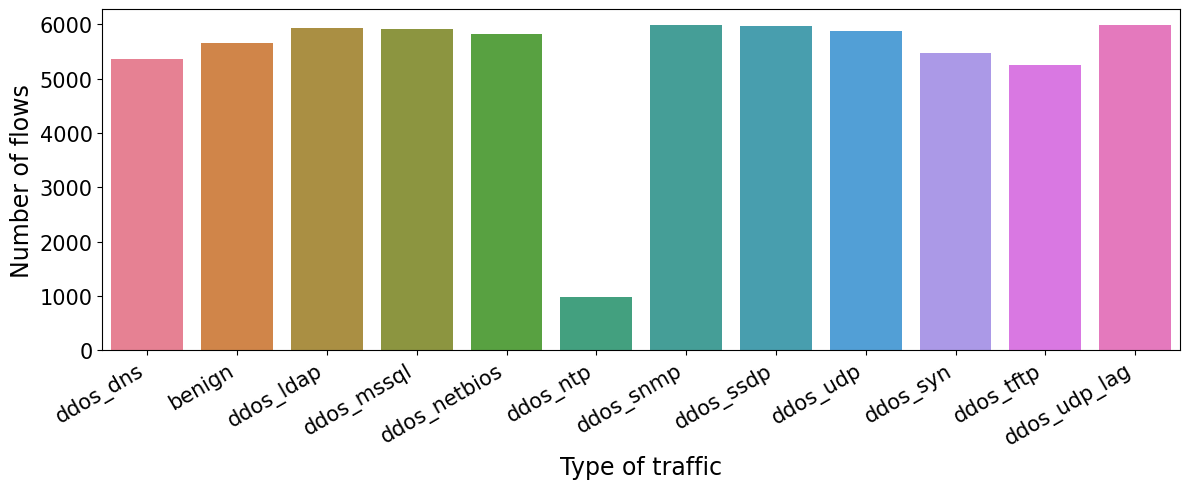
\includegraphics[width=0.8\linewidth]{img/barplot_labels.png}
		 \caption{Number of flows per label.}\label{fig:barplotLabels}
         \Description[Number of flows per label.]{}
\end{figure}

\subsection{Analysis at generic traffic level}\label{sec:featureVisualization}
In this section, we will further analyze some of the most significant features of the provided dataset, without considering the ground truth. Three different transport protocols are used: HOPOPT (\SI{0.1}{\percent} of the flows), which is the Hop-by-Hop IPv6 extension header, TCP (\SI{23.9}{\percent}) and UDP (\SI{76}{\percent}). Furthermore, the flows can be either outbound or inbound, depending on who, between the source and the destination, initialized the connection. The vast majority of them are inbound (\SI{92}{\percent}): this means that the communication is directed towards the device. In addition to this, it is also possible to analyze the most frequent destination and source IP addresses. In fact, most inbound communications (\SI{98}{\percent}) have the same destination address (192.168.50.1), while half of outbound flows have as source address 192.168.50.7. These are local IP addresses, as these attacks have been simulated in a local network. The most active links are represented in \cref{fig:barplotActiveLinks}. Definitely, the majority of the packets (\SI{90}{\percent}) are exchanged between 172.16.0.5 and 192.168.50.1. Furthermore, the flows in the dataset span all available destination ports (from 0 to \num{65535}), as shown in \cref{fig:ecdfPorts}, while the low-numbered ports are especially used by the source. 

\begin{figure}
	\centering
    \subfloat[][{Number of flows among the five most active links.}\label{fig:barplotActiveLinks}]
	{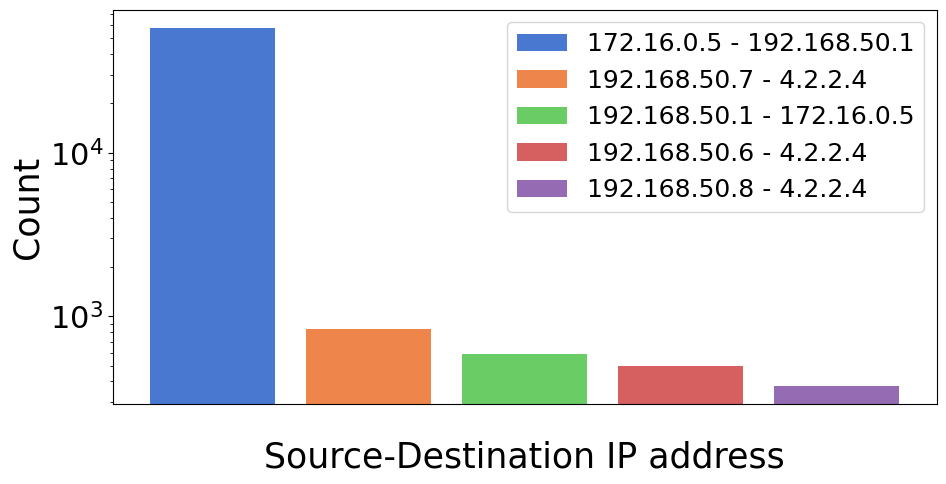
\includegraphics[width=.48\linewidth]{img/barplot_activeLinks.png}} \quad
	\subfloat[][{Port numbers distribution.}\label{fig:ecdfPorts}]
	{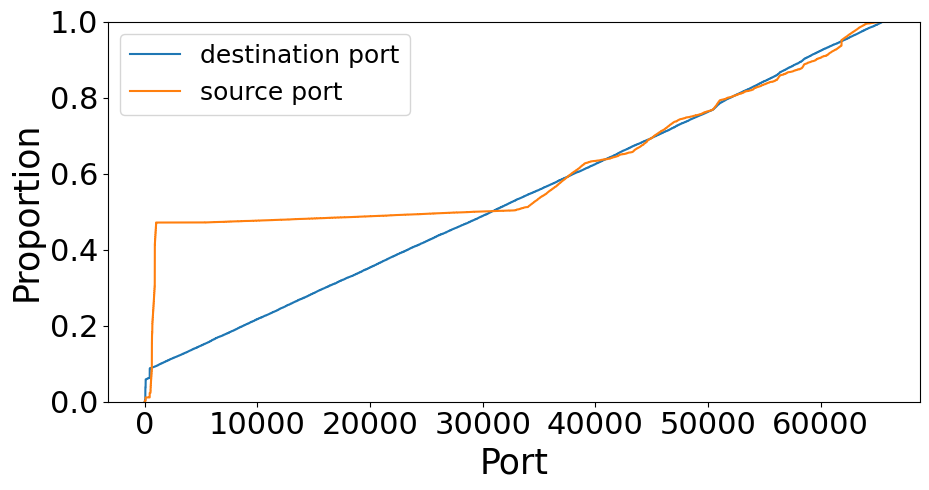
\includegraphics[width=.48\linewidth]{img/ecdf_ports.png}} \\
  	\caption{Traffic analysis based on source/destination IP address and port.} \Description[Traffic analysis based on source/destination IP address and port.]{}
\end{figure}

It is also possible to observe that the number and length of packets sent in the forward direction are usually significantly higher (up to a few hundred packets and some thousand bytes) than those sent in the backward direction. However, the goal of some of these types of DDoS attacks is to try to overload the networks by triggering big responses in the backward direction; this inconsistency may be because the reported attacks are simulated and not real ones. As expected, there is a direct proportionality between the number of packets and the total length in bytes.

According to the description of the dataset, the time features have a unit of measurement in seconds; this implies that some flows have a duration of more than three years, which is quite strange. Therefore, we will now consider them expressed in microseconds. Regardless, this assumption will not influence the subsequent steps, since the ML models do not care about the unit of measurement, as long as all the data are consistent. As a consequence, the mean flow duration is in the order of some seconds, and most of this time is idle, where the communication is not actively transferring data. On the other hand, the average inter-arrival time is in the order of a tenth of a second. There is inverse proportionality among the total number of packets and the mean IAT: therefore, the smaller this time, the more packets are sent. 

\subsection{Analysis at ground truth level} \label{sec:groundTruth}
The objective of this paragraph is to thoroughly examine the characteristics of flows belonging to the same class. In particular, we are going to start from the analysis of the timescale. In \cref{fig:lineplotAttacks}, it is possible to observe how flows are distributed during the analyzed period. Specifically, we computed the end time of each flow given its timestamp and duration, then counted the number of active flows in each interval of \SI{30}{\second}. The impulsive traffic peaks correspond to the different attacks, while the benign traffic is present along almost the entire timeline. This graph also gives some hint on the duration of the attacks: the \emph{ddos\_ntp} seems to be the longest. In \cref{fig:barplotLengthAttack} the durations of the attacks are represented, considered as the difference between the timestamp of the first sent packet and the end time of the last one. This graph confirms previous intuitions: most attacks last a couple of minutes, \emph{ddos\_ntp} is the longest one (\SI{22}{\minute}) and \emph{ddos\_snmp} is the shortest (\SI{0.8}{\second}).

\begin{figure}
	\centering
    \subfloat[][{Distribution of the traffic during the analyzed period.}\label{fig:lineplotAttacks}]
	{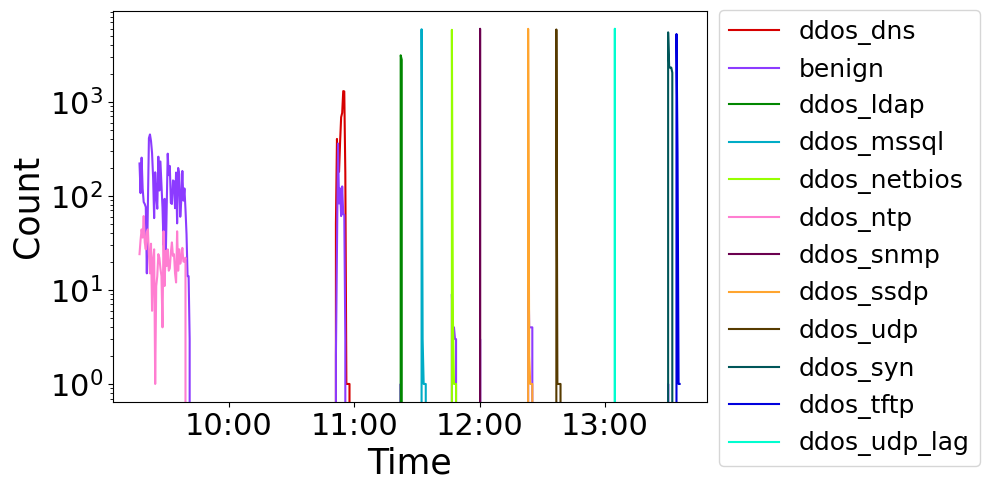
\includegraphics[width=.48\linewidth]{img/lineplot_attacks.png}} \quad
	\subfloat[][{Total attack duration per label.}\label{fig:barplotLengthAttack}]
	{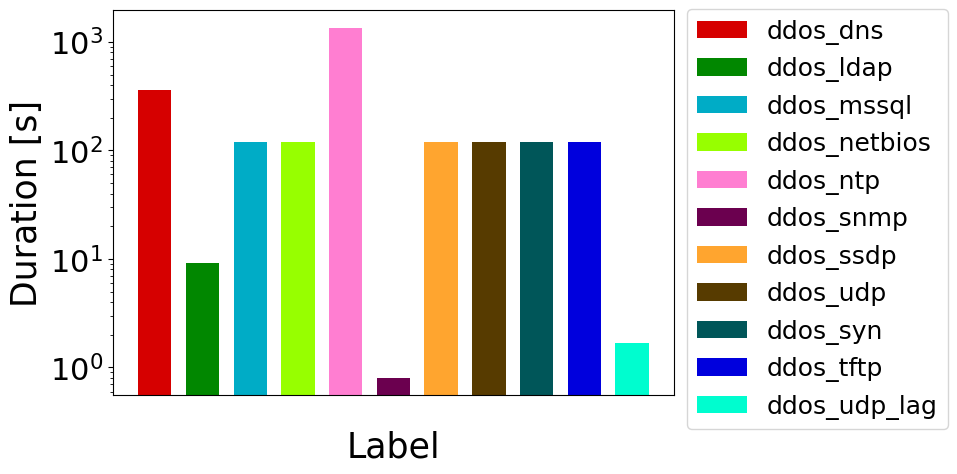
\includegraphics[width=.48\linewidth]{img/barplot_lengthAttack.png}}  \\
  	\caption{Attacks time-based analysis.}
    \Description[Attacks time-based analysis.]{}
\end{figure}

We now proceed to the analysis of the protocol employed by the various attacks. As seen before, there are three different transport protocol values in the dataset, but since the HOPOPT is used rarely and mainly by benign traffic, we will concentrate on UDP and TCP. From \cref{fig:heatmapProtocol}, it is evident that the vast majority of attacks are based on UDP; only the \emph{ddos\_syn}, the \emph{ddos\_ntp} and \emph{ddos\_tftp} flows use TCP as a transport protocol. The benign traffic is the only one fairly split among the two of them. The traffic carried on the same protocol has some common characteristics: TCP flows are usually longer, with higher active time and IAT, a comparable number of packets in the two directions, and response packets significantly bigger than the requests; in UDP, instead, the number of forward packets is a hundred times greater than the one of the backward ones. In \cref{fig:heatmapFlags}, the average number of flags per TCP flow per label is shown. It is evident that some flags (FIN, PSH, and ECE) are never used: this means that flows have used a reset packet (with the RST flag) to end the communication. Obviously, this analysis is mainly meaningful for the attack based on TCP: in each \emph{ddos\_syn} and \emph{ddos\_tftp} flow there is a packet containing the ACK flag, but not the SYN one, which is quite awkward. The \emph{ddos\_ntp} ones, instead, also employ the URG and CWE flags, which are used to tell the receiving station that the packet is urgent and that the routers are overloaded.

\begin{figure}
	\centering
    \subfloat[][{Number of flows per label per protocol.}\label{fig:heatmapProtocol}]
	{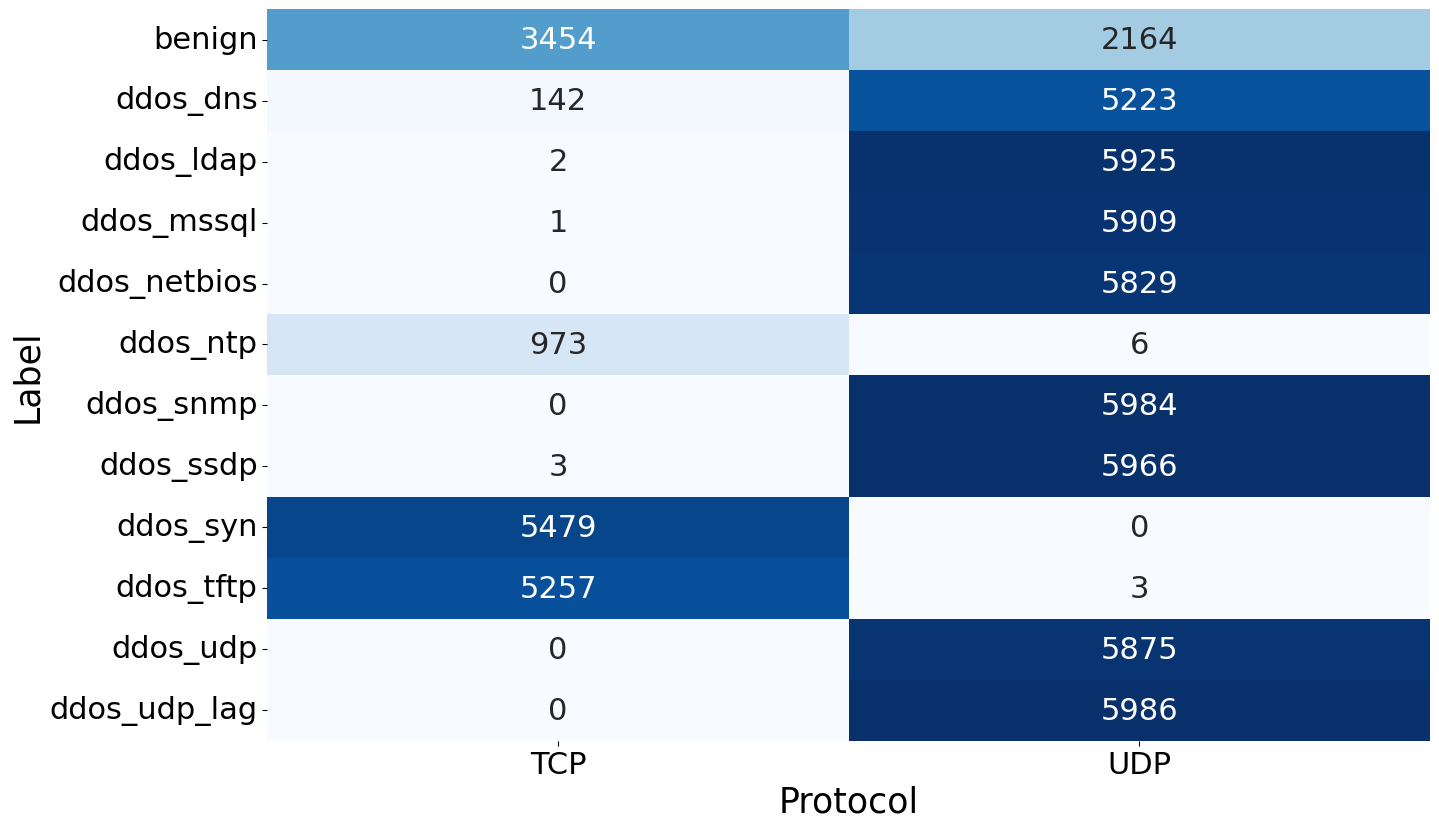
\includegraphics[width=.48\linewidth]{img/heatmap_protocol.png}} \quad
	\subfloat[][{Average number of flagged packets per flow in TCP.}\label{fig:heatmapFlags}]
	{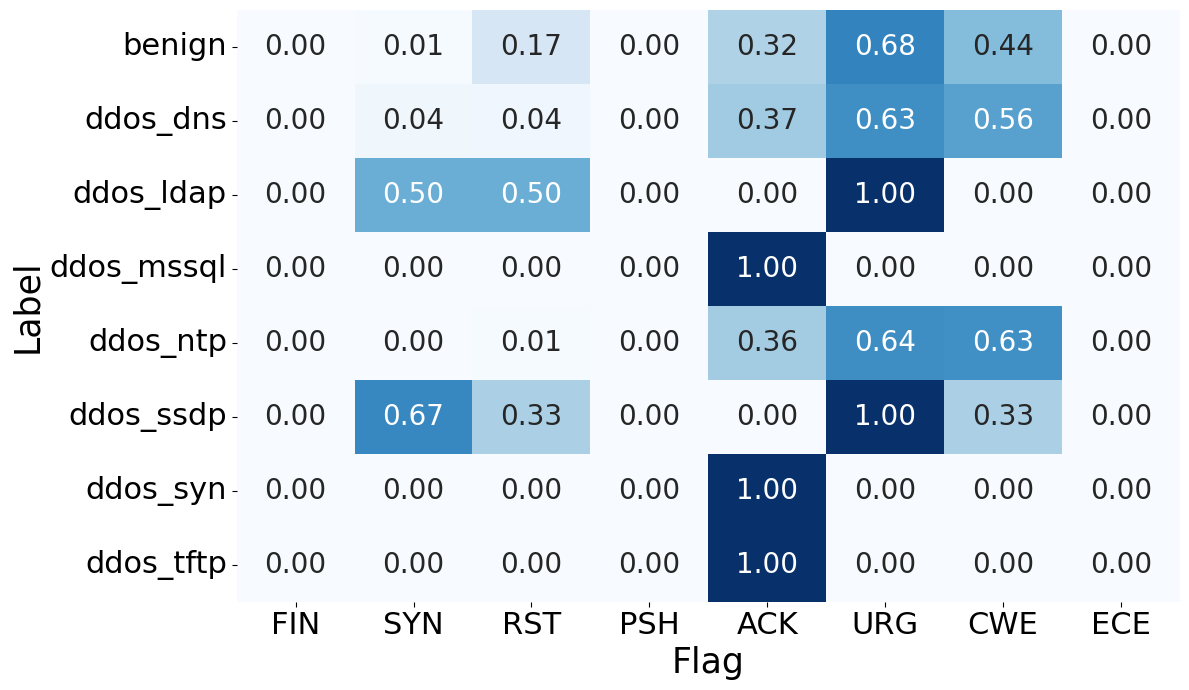
\includegraphics[width=.48\linewidth]{img/heatmap_flags.png}} \\
  	\caption{Type of protocol and flags used in the different attacks.} 
    \Description[Type of protocol and flags used in the different attacks.]{}
\end{figure}

Finally, we analyze the IP addresses and ports used. All malicious flows are between the same two IP addresses: 172.16.0.5 and 192.168.50.1. Various destination port numbers are used instead by the different kinds of attacks and protocols. As illustrated in \cref{fig:ecdfDestinationPorts}, during most of them packets are sent to several destination ports, likely to perform a port scan; only \emph{benign} and \emph{ddos\_ntp} traffic usually utilize low-numbered ports. On the other hand, the source ports used are characteristics of each attack, as shown in \cref{fig:ecdfSourcePorts}. Furthermore, most of the traffic is inbound: the only two attacks that have a significant percentage of outbound flows are \emph{ddos\_dns} (\SI{5}{\percent}) and \emph{ddos\_ntp} (\SI{30}{\percent}). Outbound traffic implies that, probably, the device has been compromised and used to carry out the attack.

\begin{figure}
	\centering
    \subfloat[][{Source ports.}\label{fig:ecdfSourcePorts}]
	{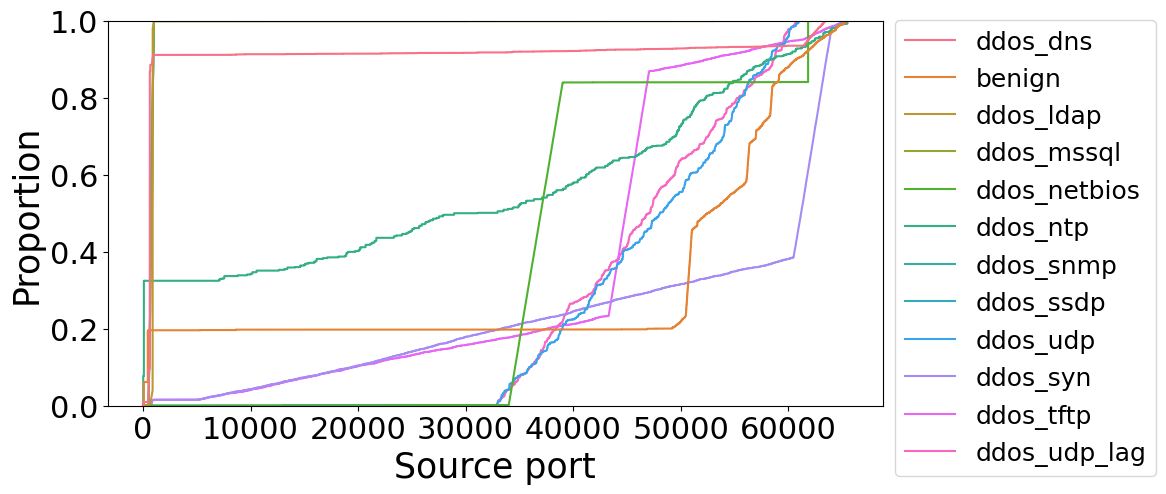
\includegraphics[width=.48\linewidth]{img/ecdf_sourcePorts.png}} \quad
	\subfloat[][{Destination ports.}\label{fig:ecdfDestinationPorts}]
	{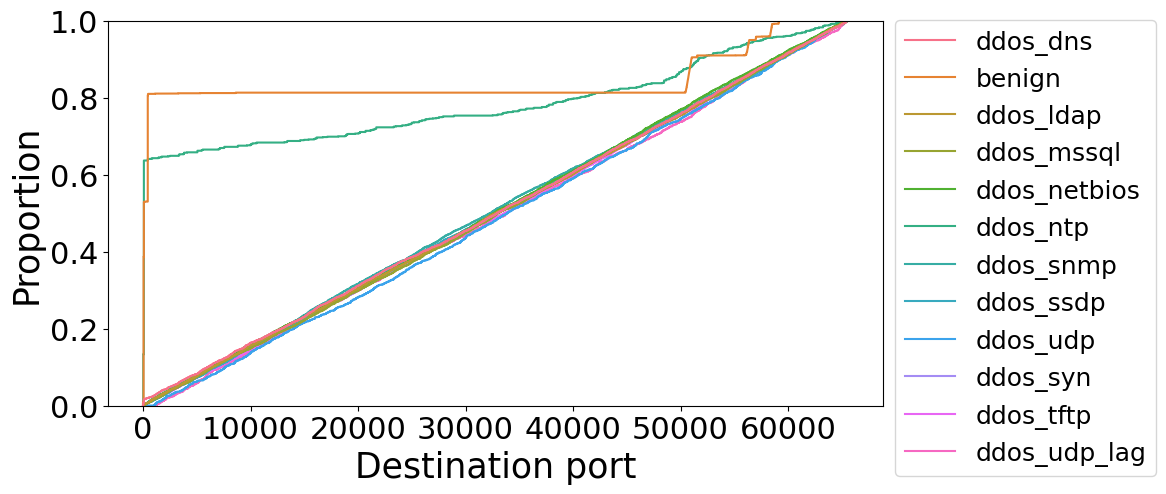
\includegraphics[width=.48\linewidth]{img/ecdf_destinationPorts.png}} \\
  	\caption{Ports used by the flows of the different attacks.} 
    \Description[Ports used by the flows of the different attacks.]{}
\end{figure}

\subsection{Additional features} \label{sec:newFeatures}
In the previous sections, we observed that the various types of attacks have different attribute values. The goal of this paragraph is to take a closer look at the most characterizing ones. To better understand which features could be the most useful for discerning the diverse classes of attacks, we used the \verb|describe| function in the \verb|pandas| library. It allowed us to compute different statistics for each feature, such as mean, maximum, minimum, quartiles, and standard deviation. 

In \cref{fig:boxplotNewFeatures}, some of the most defining features are shown. We decided to represent them as boxplots rather than histograms to highlight at the same time more characteristics of the feature: its mean, quartiles, and outliers. For visualization purposes only, we do not plot the outliers in \cref{fig:boxplotFwdPackets} and in \cref{fig:boxplotPacketLength}, because they are higher orders of magnitude than most data. 

\begin{figure}
	\centering
    \subfloat[][{Flow Duration.}\label{fig:boxplotFlowDuration}]
	{\includegraphics[width=.48\linewidth]{img/boxplot_FlowDuration.png}} \quad
	\subfloat[][{Flow Bytes/s.}\label{fig:boxplotFlowBytes}]
	{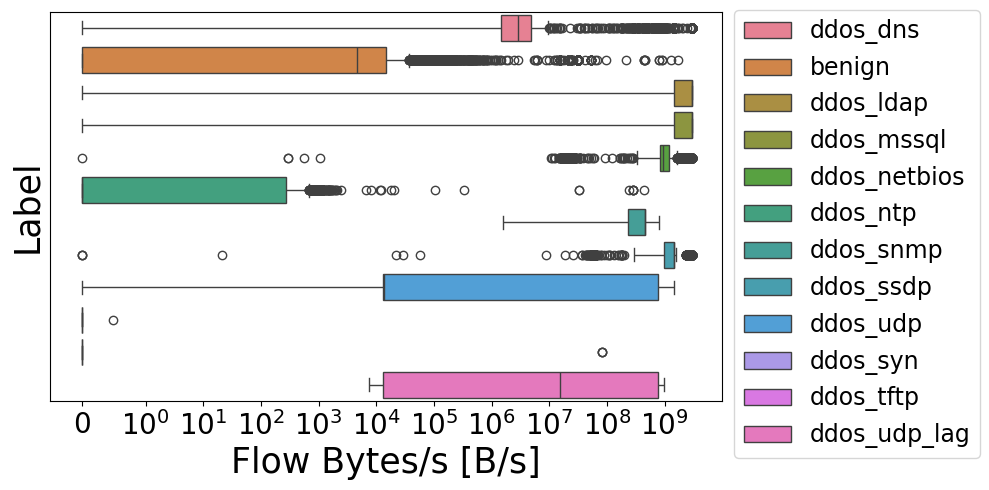
\includegraphics[width=.48\linewidth]{img/boxplot_FlowBytes.png}} \\
    \subfloat[][{Total number of forwarded packets.}\label{fig:boxplotFwdPackets}]
	{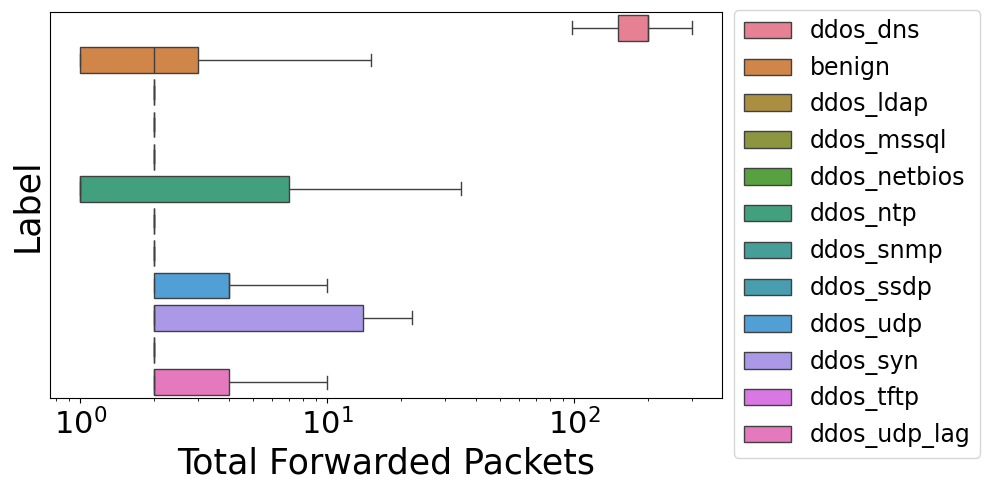
\includegraphics[width=.48\linewidth]{img/boxplot_totalFwdPackets.png}} \quad
	\subfloat[][{Mean of packets length.}\label{fig:boxplotPacketLength}]
	{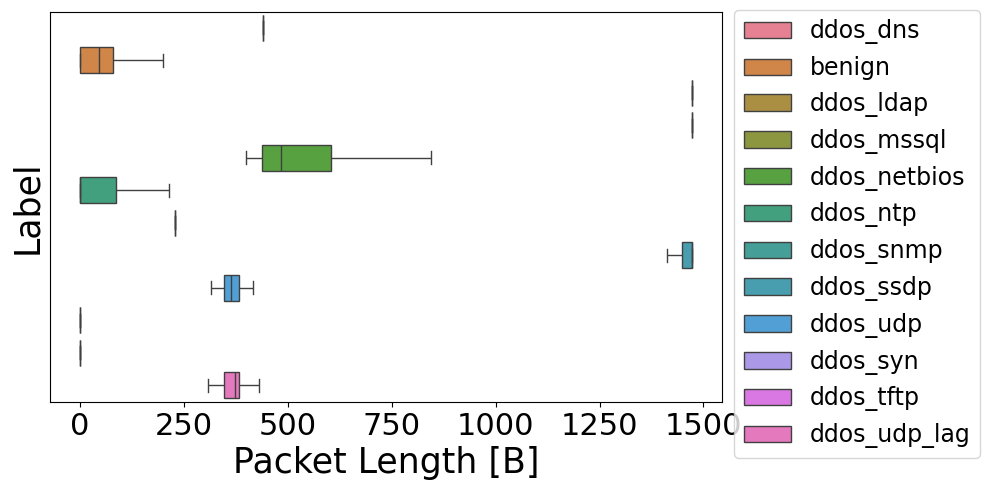
\includegraphics[width=.48\linewidth]{img/boxplot_packetLength.png}} \\
  	\caption{Attack characterizing features.} 
    \Description[Attack characterizing features.]{}\label{fig:boxplotNewFeatures}
\end{figure}

In \cref{fig:boxplotFlowDuration} the flow duration feature is illustrated. In particular, some attacks have flows that can last a very different amount of time (i.e, \emph{ddos\_ntp}, \emph{ddos\_udp}, \emph{ddos\_syn}, and \emph{ddos\_udp\_lag}). Some, in contrast, are usually very short (i.e., \emph{ddos\_ldap}, \emph{ddos\_mssql}, \emph{ddos\_snmp}, and \emph{ddos\_ssdp}) with outliers that last longer. \emph{ddos\_tftp} flows have a duration of up to a few hundred microseconds, while \emph{ddos\_dns} and \emph{benign} tend to be longer, but have many more lengthy outliers. Moreover, we noticed that the inter-arrival time values follow approximately the same pattern.

In \cref{fig:boxplotFlowBytes} the flow rate is represented: some attacks, such as \emph{ddos\_ldap}, \emph{ddos\_mssql}, \emph{ddos\_netbios}, \emph{ddos\_snmp}, and \emph{ddos\_ssdp}, have a very high and consistent one, while for \emph{ddos\_syn} and \emph{ddos\_tftp} it is almost zero, with very few outliers. The flows of the other attacks have a more variable rate.

The number of forwarded packets, shown in \cref{fig:boxplotFwdPackets}, allows us to distinguish \emph{ddos\_dns} flows from all the others, since they are significantly the ones with the highest number. However, other types of traffic, such as \emph{benign} one, have outliers with a higher number of packets sent. Backward traffic can also be helpful in classifying the types of attacks, as only \emph{benign} and \emph{ddos\_ntp} flows send many backward packets.

Concerning \cref{fig:boxplotPacketLength}, we can notice that each class of attack has its own specific packet length, even though there are smaller or larger outliers. \emph{benign}, \emph{ddos\_ntp}, \emph{ddos\_syn}, and \emph{ddos\_tftp} have usually little packets (less than \SI{100}{\byte}), while \emph{ddos\_ldap}, \emph{ddos\_mssql}, and \emph{ddos\_ssdp} ones are very big. The other attacks, finally, send packets of intermediate length. 

From this analysis, it is clear that some attacks tend to have common characteristics. For instance, a group could be composed of \emph{ddos\_ldap},  \emph{ddos\_mssql}, \emph{ddos\_snmp}, and \emph{ddos\_ssdp} flows, another by \emph{ddos\_udp} and \emph{ddos\_udp\_lag}, and a last one by \emph{ddos\_syn} and \emph{ddos\_tftp}. Also \emph{benign} and \emph{ddos\_ntp} are quite similar. 

We decided not to add new features based on these metrics to the dataset, otherwise we would replicate the same values across all rows classified with the same label. Hence, we would pass the label indirectly to our ML models, which would certainly lead to high accuracy but not very meaningful results. Moreover, in a real-world scenario, we would not be able to add these new features to new flows we want to classify since we do not yet know the label.

\subsection{Correlation analysis} \label{sec:correlationAnalysis}
This step explores the relationships between the different numerical features. ML algorithms are sensitive to data and if two features are highly correlated, it might be that one of them is redundant, because the information provided is already replicated. If an ML model is trained using both features, it will essentially learn the same information from both, which is not only unnecessary but also increases model complexity, potentially leading to higher computational costs. To analyze the correlations, we visualize a heatmap of the correlation matrix, which highlights relationships between features. This was done using two metrics: Pearson's correlation coefficient (for linear relationships) and Spearman's rank correlation (for monotonic relationships, hence not necessarily linear). These metrics provide a quantitative assessment of the strength of the correlation and are useful in guiding feature selection decisions. We observed some slight differences among the two correlation matrices visualized: for example, according to the Pearson's correlation coefficient the flow IAT and the idle time are strongly correlated, while that is not true according to the Spearman's one. Furthermore, we can deduce that there is a non-linear relationship between the idle and the active time. On the other hand, the IAT and the flow duration are strongly correlated according both coefficients. Finally, we can notice that the different metrics about the IAT are strongly correlated. The correlation matrix computed using Pearson's coefficient is shown in \cref{app:correlationMatrix}.

\subsection{Label encoding} \label{sec:labelEncoding}
Label encoding is a discretization technique that is usually applied to an attribute to convert its values from any domain to a numerical one. This is particularly useful for categorical features that, due to their nature, cannot be directly interpreted by ML models.

After careful analysis, we decided to apply label encoding exclusively to the feature \emph{Protocol}, as the protocol associated with various flows is relevant to our task, as demonstrated in \cref{sec:groundTruth}. Moreover, the \emph{Protocol} feature contains a very small set of numerical values (only three), so we apply the label encoding because the model might misinterpret these values as having an ordinal relationship or magnitude, whereas in reality, no such order exists among the protocols. However, this encoding has little impact on the performance of the models that we trained in \cref{sec:supervisedLearning}. 

Regarding the choice of a label encoding technique, there are several options. For instance, one-hot encoding creates a separate binary column for each category, which can be useful but may significantly increase the number of columns, especially for features with a wide range of values. In our case, we applied this technique because the \emph{Protocol} feature has a very small set of values. This approach provides an efficient and straightforward representation without introducing too much complexity.

On the other hand, for other categorical features such as \emph{Source Port} or \emph{Destination Port}, applying label encoding would not be appropriate due to the wide range of possible values. Furthermore, a wide range of values could increase the risk of overfitting and reduce the model's ability to generalize, further justifying our choice. 

We faced the same issue for the IP source and destination addresses: they are categorical features that cannot be interpreted by ML models, but they seem significant to discern the traffic. Since there are too many possible values to perform label encoding, we decided to transform them into their binary representation (they are composed of four bytes). However, we experimented as the performance of ML models remained the same even removing those features.

In addition, we decided to simply ignore the remaining categorical features for the following reasons:
\begin{itemize}
    \item \emph{Flow ID}: it does not bring any relevant information since it is composed of the IP quintuple that is already present in other features.
    \item \emph{Similar HTTP}: its value is zero in more than the \SI{99}{\percent} of the cases, so it is not very significant.
    \item \emph{Timestamp}: we tried to transform it into its representation in seconds and then train the ML models described in \cref{sec:supervisedLearning}. Their performance on this specific dataset definitely increased, but our models should also be applicable to discern future attacks, so the timestamp might be in another interval of time, leading to wrong classifications.
\end{itemize}

\subsection{PCA} \label{sec:PCA}
\begin{figure}
	\centering
		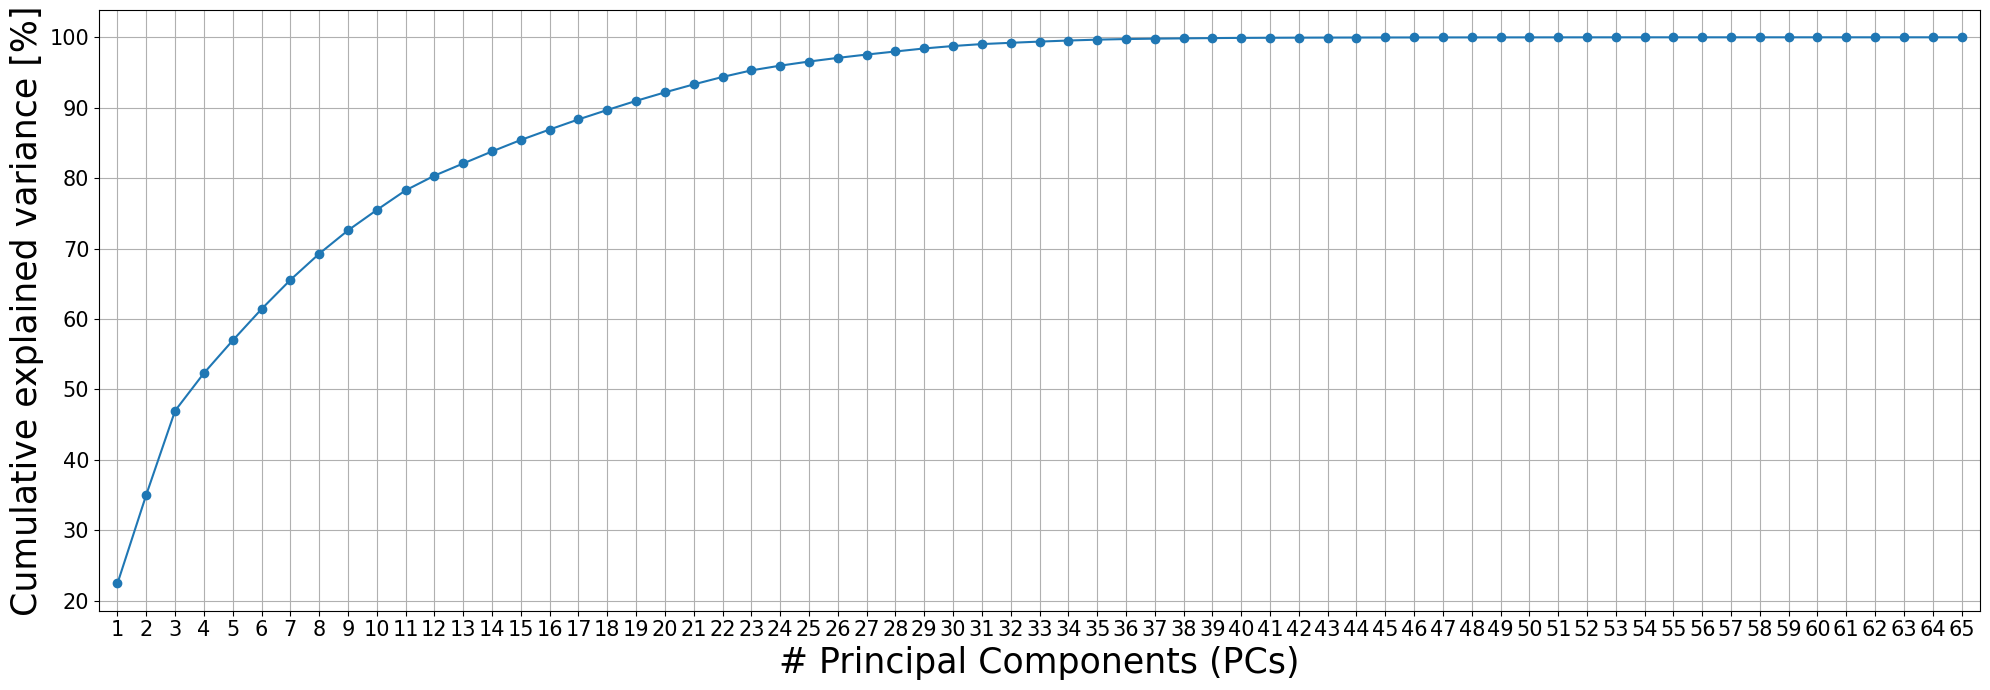
\includegraphics[width=1\linewidth]{img/PCAElbowMethod.png}
		 \caption{PCA: elbow method.}\label{fig:PCA}
         \Description[PCA: elbow method.]{}
\end{figure}
Principal Component Analysis (PCA) is a technique used to project the original dataset into a new feature space (the components). It reduces the number of variables while preserving the core characteristics and variations of the dataset as much as possible. We perform PCA because it is particularly useful for high-dimensional datasets, since it can simplify the dataset management, speed up the training process, and improve model generalization by mitigating the risk of overfitting.

The data require a standardization process, as PCA assumes that all features are on the same scale. Without standardization, features with larger magnitudes could disproportionately affect the explained variance, therefore misleading the outcome. By standardizing, we ensure that all features contribute equally to the variance analysis, allowing PCA to effectively identify the principal components useful for our ML task. In this case, 40 Principal Components are enough for our dataset, as they explain \SI{99.92}{\percent} of the cumulative variance. The elbow method chart is illustrated in \cref{fig:PCA}.

\subsection{Analysis of the features obtained via PCA} \label{sec:PC}
In this section, we will examine the new features obtained via PCA. As expected, the resulting components are no longer correlated with each other, which is one of the most important advantages of this technique.

\Cref{fig:ecdfPC} shows the empirical cumulative density functions (ECDF) of the first two principal components. Each class of attack has a different trend, but we can recognize the same similarities we identified at the end of \cref{sec:newFeatures}. In fact, in both graphs the lines of \emph{ddos\_ldap} and \emph{ddos\_mssql}, and the ones of \emph{ddos\_udp} and \emph{ddos\_udp\_lag} are almost overlapped; the ones of \emph{ddos\_syn} and \emph{ddos\_tftp}, instead, are slightly different: the former has a slower increase, which implies that, for PC1, there are no values between 2 and 10. These patterns can be found in all the generated principal components: the main difference is that, while for the first ones the range of possible values is quite wide (approximately between -5 and 20), for the last ones it is pretty narrow (between -0.5 and 0.5). As a consequence, ML models may misclassify the samples of these classes due to their very similarity. This issue will be further investigated in the following sections.

\begin{figure}
	\centering
    \subfloat[][{ECDF of the first principal component.}\label{fig:ecdfPC1}]
	{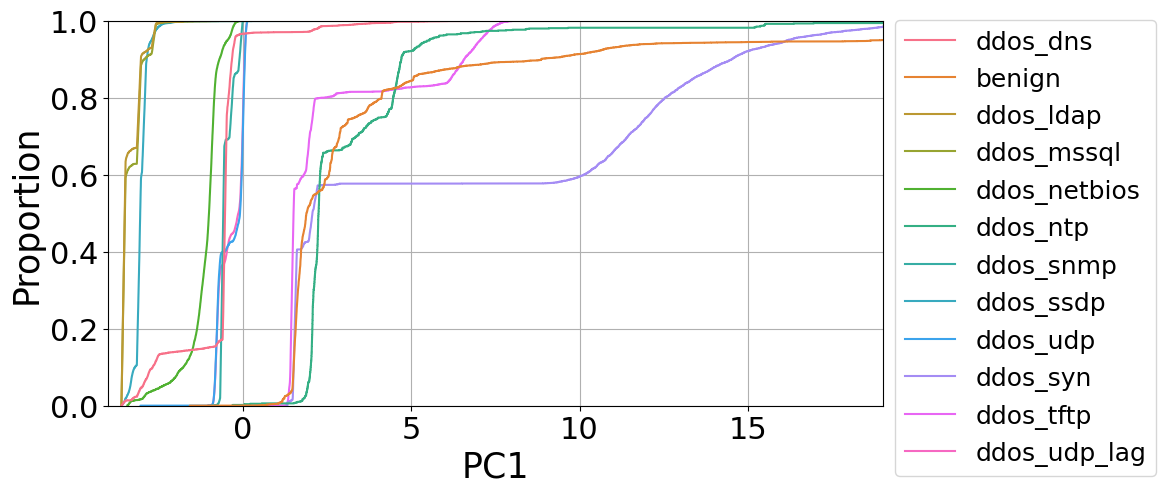
\includegraphics[width=.48\linewidth]{img/ecdf_PC1.png}} \quad
	\subfloat[][{ECDF of second principal component.}\label{fig:ecdfPC2}]
	{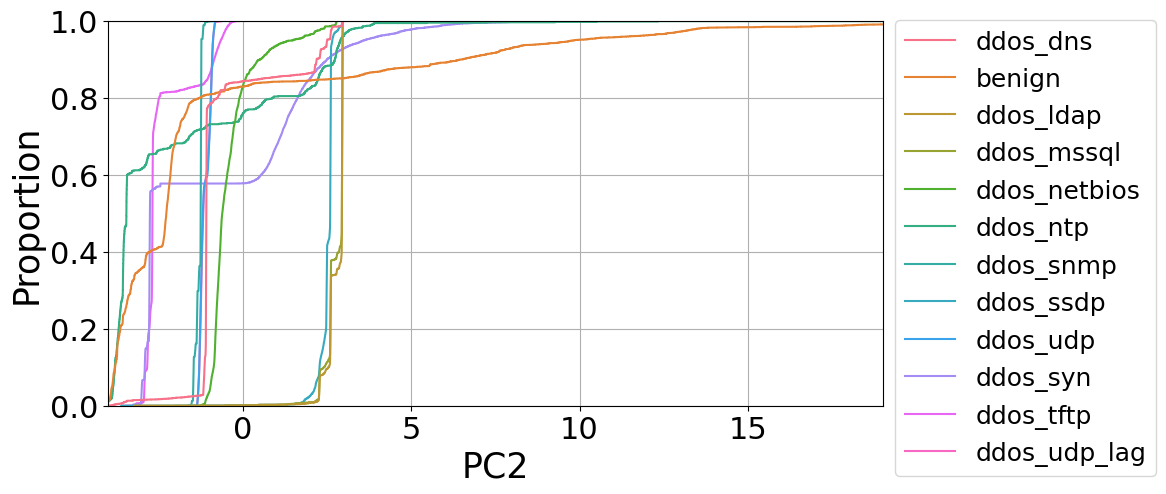
\includegraphics[width=.48\linewidth]{img/ecdf_PC2.png}} \\
  	\caption{ECDF of the first two principal components.} 
    \Description[ECDF of the first two principal components.]{}\label{fig:ecdfPC}
\end{figure}

Finally, we analyzed the loading scores of the first two principal components. In particular, PC1 strongly depends on the inter-arrival and idle time, while PC2 is mainly affected by the maximum packet length.

\subsection{Removing correlated features}\label{sec:removeCorretedFeatures}
One of the main disadvantages of PCA is that it limits the interpretability of the features obtained and, as a consequence, the results that we obtain from the ML models. For this reason, after standardizing our dataset, we decided to perform dimensionality reduction by removing the columns that have a correlation greater than \num{0.8} in absolute value. In doing so, we removed 36 features and kept 29 of them, without considering the ones we already dropped for the reasons explained in the previous sections. We will apply both supervised and unsupervised ML techniques to this reduced dataset, as there is no big difference in performances compared to that obtained using PCA components. Moreover, we also verified that there is no performance decrease when using the simplified dataset rather than the original one.

\section{Supervised learning – classification} \label{sec:supervisedLearning}
The goal of this part is to classify the flows into different types of attacks based on the features retained in the dataset. This section focuses on selecting different models, training and testing them with default parameters, and performing hyperparameter tuning to evaluate whether the optimization process yields improvements and significant results.  

\subsection{Dataset pre-processing}
\subsubsection{Train test split}
First, it is essential to split the dataset into training and test sets. This split must be performed in a stratified manner with respect to the labels to ensure a balanced distribution of samples across all classes. This approach is crucial to achieving reliable results and mitigating the risks of overfitting or underfitting. 

\subsubsection{Data preparation}
Then, we pre-processed our dataset as explained in the previous paragraphs. In particular, we removed inconsistent and categorical features, performed the encoding as explained in \cref{sec:labelEncoding}, scaled our dataset and dropped highly correlated features (\cref{sec:removeCorretedFeatures}). In this case, however, we fit the \verb|StandardScaler| and computed the correlation only on the training set, then transformed both the training and the test sets: this ensures that the model's evaluation on the test set remains fair and realistic. We also transformed class labels into integers using the \verb|LabelEncoder| since some ML algorithms work only with numerical labels.

\subsection{Classification algorithms}
\subsubsection{ML models}
At this point, we trained the models with the default parameters to pick, among the ones presented during the course, the most suitable to our dataset. The chosen ones are the following:
\begin{itemize}
    \item k-Nearest Neighbors (k-NN): An algorithm that classifies a sample based on the majority class of its nearest neighbors.
    \item Logistic Regression: A linear model commonly used for binary and multiclass classification that predicts the probability that a sample belongs to a specific class and is particularly effective when the relationship between features is approximately linear.
    \item Random Forest: An ensemble learning method based on decision trees. It combines multiple trees to improve accuracy, making it robust for datasets with complex, nonlinear relationships.
\end{itemize}
To read more about the two discarded models (Naive Bayes and Support Vector Machines), refer to \cref{app:otherModels}. 

\subsubsection{Hyperparameter tuning}
Next, we performed the hyperparameter tuning to find the best combination that leads to the highest accuracy on the validation set. To this end, we used the \verb|GridSearchCV| function provided in the \verb|sklearn.model_selection| library. It performs stratified 5-fold cross-validation and can exploit all the cores of the PC if the \emph{n\_jobs} parameter is set to -1. As a result, the computation is much faster than with a custom implementation.

\subsubsection{Preliminary remarks}\label{sec:preliminaryRemarks}
We observed some common behaviors among the ML algorithms. In particular, the performance varies between the different types of attack (classes), and this can be attributed to several factors. In fact, some classes have feature values that are more distinct, such as \emph{benign}, \emph{ddos\_dns}, \emph{ddos\_syn}, and \emph{ddos\_tftp} ones, leading to high precision, recall, and F1-scores. Other attack types, instead, have overlapping features, making it harder for the models to distinguish between such classes. For example, we saw in \cref{sec:newFeatures} and \cref{sec:PC} that \emph{ddos\_ldap},  \emph{ddos\_mssql}, and \emph{ddos\_ssdp} flows have some common characteristics (e.g., flow duration, transmission rate, and packet length) and also \emph{ddos\_udp} and \emph{ddos\_udp\_lag} may be difficult to discern. Furthermore, certain attacks (e.g., \emph{ddos\_mssql}, \emph{ddos\_snmp}) have features that are noisier or less discriminative, leading to poorer precision and recall.

\subsection{First model: k-Nearest Neighbors (k-NN)}
\subsubsection{Default model performance evaluation} 
The model achieves higher accuracy (\SI{86}{\percent}) in the training set compared to the test set (\SI{79}{\percent}). This difference may indicate a little overfitting, meaning that the model is too tailored to the training data and does not generalize well to unseen data. 

Most classes have high precision and recall in the training set, while some of them perform worse in the test set. In particular, \emph{ddos\_mssql}, \emph{ddos\_udp} and \emph{ddos\_udp\_lag} have a precision higher than \SI{70}{\percent} in the training set, which drops to around \SI{55}{\percent} in the test. The \emph{ddos\_ldap} class is the one in which the model performs worst, suggesting that it is not able to generalize such attack.

\subsubsection{Hyperparameter tuning} 
An effective strategy to enhance model performance is to perform hyperparameter tuning to find the best possible combination of values for the model parameters. In the k-NN model, we decided to optimize the following parameters:
\begin{enumerate}
    \item \emph{n\_neighbors}: this is one of the most important parameters for this model. A too-low value makes the model sensitive to noise (overfitting), while a too-high value can reduce the importance of the most relevant neighbors (underfitting).
    \item \emph{weights}: with \verb|uniform|, each neighbor has the same weight; with \verb|distance|, the nearest neighbors are given more weight, which can be useful for optimization.
    \item \emph{p}: this specifies the type of distance used in neighbor detection: with $\emph{p}=1$, the Manhattan distance is used, while with $\emph{p}=2$, the Euclidean distance is used.
\end{enumerate}
We did not test different algorithms to compute the nearest neighbors, as the \verb|auto| option already attempts to identify the most appropriate algorithm based on the values passed to the fit method.

\subsubsection{Results} 
\Cref{fig:hyperparamKNN} shows the accuracy in the training and validation sets with respect to different parameter configurations. In particular, we noticed that, in general, the model works better with \emph{p} set to 1 (Manhattan distance). The combination of hyperparameters that leads to the best accuracy in the validation set (\SI{80}{\percent}) is $\emph{n\_neighbors}=6$, $\emph{weights}=\verb|distance|$, and $\emph{p}=1$. As a result, we obtain an accuracy of \SI{100}{\percent} in the training set: our model is probably overfitting. However, we obtained similar accuracy values in the validation set even with other combinations of hyperparameters (using $\emph{weights}=\verb|uniform|$) that lead to a lower accuracy (around \SI{85}{\percent}) in the training set.

Several factors can contribute to overfitting. For example, k-NN, especially with a small number of neighbors considered, tends to memorize the training data, making it highly sensitive to noise and outliers. However, this is probably not our case since we considered 6 of them. Additionally, high dimensionality also influences the results: if the dataset has many features, the ``curse of dimensionality'' makes distance calculations less meaningful. This affects the ability of k-NN to classify accurately.

Regarding the training cost of the model, we believe that the time spent performing the hyperparameter tuning is not really a meaningful metric to compare the different models because it may vary according to the number of values tested. On the other hand, we can consider the time to perform the fit on the training set and the predict on the whole dataset as a more relevant indicator of the model's cost, even if it is machine-dependent. The fit of the k-NN model takes \SI{0.01}{\second}, while the predict takes \SI{11.25}{\second}. In fact, it does not construct a general internal model, but simply stores the instances of training data. Then, during the predict phase, it computes the distances between the records to find the closest neighbors.

\begin{figure}
	\centering
    \subfloat[][{Grid search k-NN.}\label{fig:hyperparamKNN}]
	{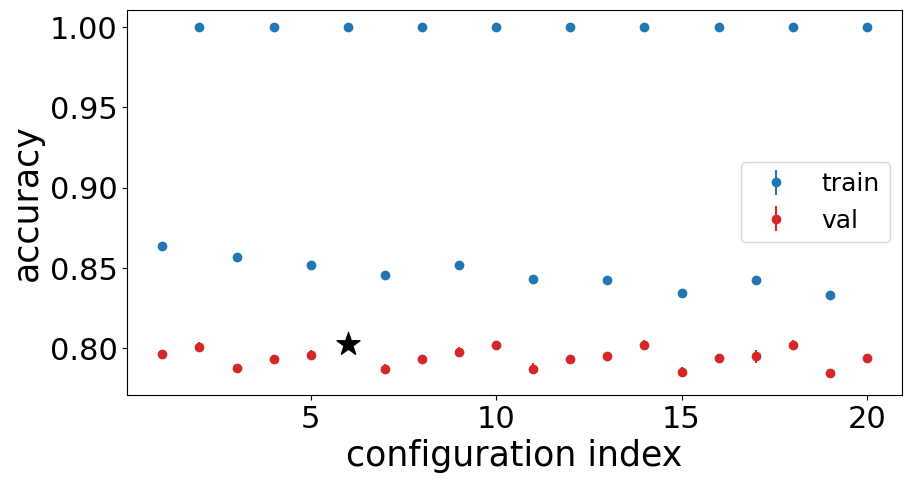
\includegraphics[width=.48\linewidth]{img/hyperparam_KNN.png}} \quad
	\subfloat[][{Grid search Logistic Regression.}\label{fig:hyperparamLR}]
	{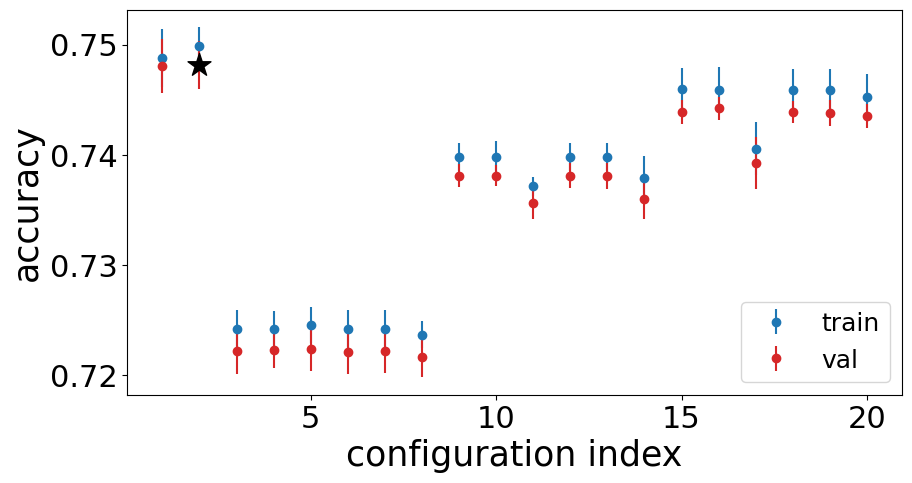
\includegraphics[width=.48\linewidth]{img/hyperparam_LR.png}} \\
  	\caption{Hyperparameter tuning k-NN and Logistic Regression models.} 
    \Description[hyperparameter tuning k-NN and Logistic Regression models.]{}
\end{figure}

\subsection{Second model: Logistic Regression}
\subsubsection{Default model performance evaluation} 
Logistic Regression assumes that the data is linearly separable, so if the features of some attacks are not, the model struggles to classify them (e.g., \emph{ddos\_mssql}). Moreover, logistic regression cannot model complex relationships between features, meaning that its simplicity can result in poor classification performance when there are intricate patterns in certain attacks.

The model exhibits an accuracy (\SI{74}{\percent}) in both the training and test sets. Since the performance is acceptable and the two sets have similar accuracy, we cannot detect overfitting or underfitting. Using the default parameters, the model is not able to converge, which means that it was still learning when it reached the maximum number of iterations.

\subsubsection{Hyperparameter tuning} 
We optimized the following parameters:
\begin{enumerate}
    \item \emph{solver}: algorithm to use in the optimization problem. For multiclass problems, we can use the \verb|lbfgs|, \verb|newton-cg| and \verb|saga| solver. Since the model did not reach convergence even after a high number of iterations with the last solver, we decided to use the first two.
    \item \emph{penalty}: it specifies the norm of the penalty. If set to \verb|None| no penalty is added; while with \verb|l2| a L2 penalty term is added.
    \item \emph{C}: inverse of regularization strength; as in support vector machines, smaller values specify stronger regularization.
    \item \emph{tol}: tolerance for stopping criteria.
\end{enumerate}
\emph{C} and \emph{tol} can only be set if \emph{penalty} is set to \verb|l2|.

\subsubsection{Results}
The combination of hyperparameters that leads to the highest accuracy in the validation set (\SI{75}{\percent}) is \emph{solver}=\verb|newton-cg| and \emph{penalty}=\verb|None|. Since the accuracy in the training set is very similar, there is no overfitting. \Cref{fig:hyperparamLR} shows the results of the performed grid search. In particular, we can notice that some combinations, with \emph{penalty}=\verb|l2| and a low value of \emph{C}, lead to lower accuracy than others.

Among the three models analyzed here, Logistic Regression is the one with the highest cost: the fit phase takes \SI{46.91}{\second}, since it has to build the model. The predict, instead, is very short, just \SI{0.01}{\second}.

\subsection{Third model: Random Forest} 
\subsubsection{Default model performance evaluation} 
The model achieves excellent performance (\SI{100}{\percent}) in the training set. Although the performance on the test set is high (\SI{86}{\percent} accuracy), the gap between training and test accuracy suggests that the model is memorizing the training data rather than generalizing well to unseen data, which is a clear indication of overfitting. In particular, looking at the default parameters, we discovered that the tree nodes are expanded until all leaves are pure, so it may be too strongly affected by the training data. We will address this issue in the hyperparameter tuning phase. Furthermore, all metrics (precision, recall, F1-score) are 1.00 for every class in the training set, but some classes, such as \emph{ddos\_mssql}, \emph{ddos\_udp}, and \emph{ddos\_udp\_lag}, show a marked drop in performance in the test set. 

\subsubsection{Hyperparameter tuning} 
For the Random Forest model, we optimized the following parameters:
\begin{enumerate}
    \item \emph{n\_estimators}: this represents the number of trees in the forest. A value that is too low may result in underfitting, while an excessively high value increases training time without significant performance improvements.
    \item \emph{max\_depth}: the maximum depth of the trees. Excessive depth can lead to overfitting, while insufficient depth may cause underfitting.
    \item \emph{min\_samples\_leaf}: the minimum number of samples required to be at a leaf node. A number that is too low may cause overfitting.
    \item \emph{criterion}: the function used to measure the quality of a split. Optimizing this parameter can enhance the model's performance.
\end{enumerate}

\subsubsection{Results} 
The results of the grid search performed are shown in \cref{fig:hyperparamRF}. It is evident that with some combinations we obtained lower accuracies, around \SI{80}{\percent}: these cases are the ones in which the depth of the trees is up to 5, which is definitely not enough. Moreover, increasing the number of trees does not bring any advantage in terms of performances, only more costs. In general, the best performances are obtained using $\emph{max\_depth}=15$: it is better not to completely expand all the nodes, as it may lead to overfitting. Trying to run the hyperparameter tuning multiple times, we obtained different best combinations, since the performance variations are very slight and they may be affected by the split selected. For this reason, we chose one of the least computationally expensive, since it is based on a low number of estimators.

The combination of hyperparameters that leads to the best accuracy in the validation set (\SI{87}{\percent}) is: $\emph{n\_estimators}=50$, $\emph{max\_depth}=15$, $\emph{min\_samples\_leaf}=1$, and $\emph{criterion}=\verb|gini|$. In this case, we obtained an accuracy of \SI{90}{\percent} in the training set: since both sets have a similar accuracy value, there is no more overfitting. Our model still performs better in some classes than in others, having a precision of only \SI{62}{\percent} in the test set in \emph{ddos\_udp} and \emph{ddos\_udp\_lag}.

Regarding the costs, we measured that the fit takes \SI{1.38}{\second}, while the predict phase \SI{0.22}{\second}. During the fit phase, in fact, the model creates the decision trees, while during the predict phase it simply compares the features values with the ones in the nodes to choose the best path for that sample.

\begin{figure}
	\centering
    \subfloat[][{Grid search Random Forest.}\label{fig:hyperparamRF}]
	{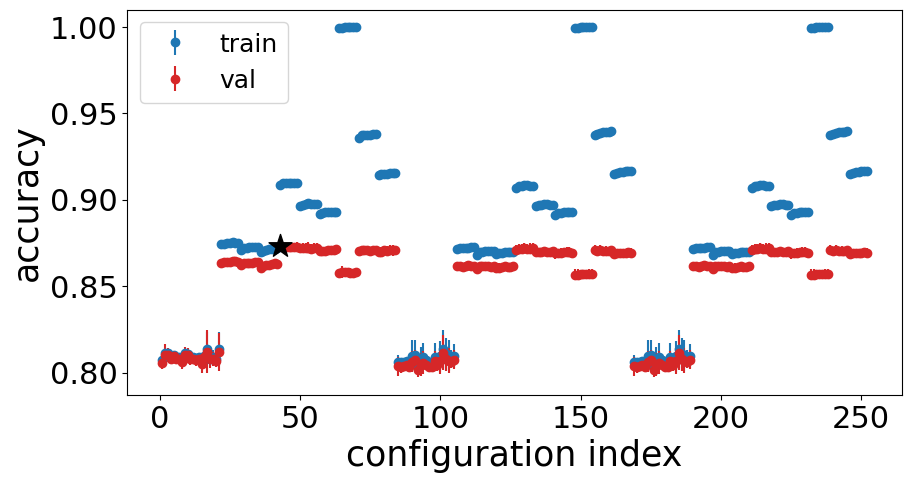
\includegraphics[width=.48\linewidth]{img/hyperparam_RF.png}} \quad
	\subfloat[][{Learning curve Random Forest.}\label{fig:learningCurve}]
	{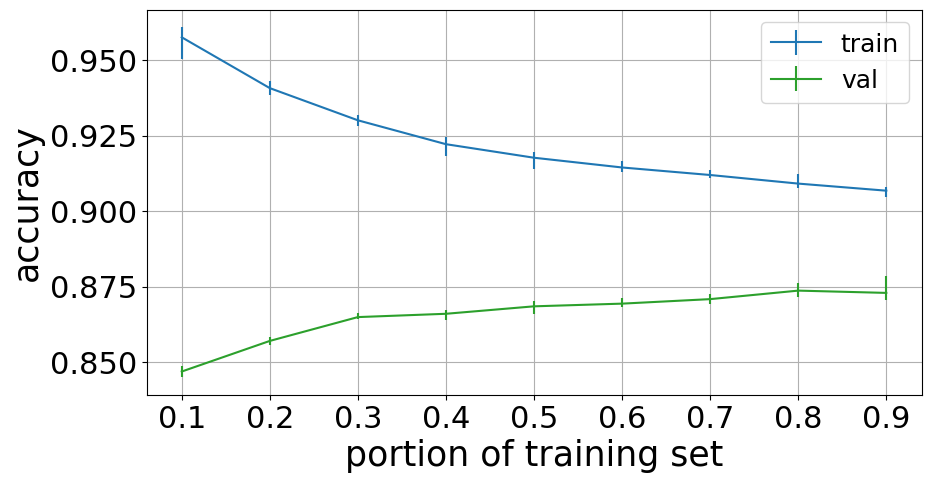
\includegraphics[width=.48\linewidth]{img/learningCurve.png}} \\
  	\caption{Hyperparameter tuning on Random Forest model.} 
    \Description[hyperparameter tuning on RF model]{}
\end{figure}

\subsection{Selection of the best model}
This final step involves selecting the model that shows the best performance in multiple metrics. By analyzing the classification report of all the models in both the training and test sets, it is evident that the Random Forest and k-NN models outperform Logistic Regression. Furthermore, Random Forest is generally more effective than k-NN in several metrics, making it the better choice:
\begin{enumerate}
    \item Higher test accuracy: Random Forest achieves \SI{87}{\percent} accuracy, compared to \SI{80}{\percent} for k-NN.
    \item Better Macro and Weighted Averages: Random Forest has a macro average F1-score of 0.88, while k-NN achieves 0.81.
    \item Consistent Precision and Recall: Random Forest maintains higher and more consistent precision and recall values in the test set for most classes, ensuring fewer false positives and false negatives.
\end{enumerate}

As for the costs, it is clear that Logistic Regression is the least efficient. Random Forest is slower during the fit phase than during the predict one, while for k-NN, it is the opposite. However, in a real-world scenario, we would like to train our model and then efficiently and rapidly predict labels for new data. For this reason, we would prefer Random Forest rather than k-NN.

In conclusion, we do believe that Random Forest is the best model because it generalizes better to unseen data, provides higher accuracy, and demonstrates superior precision, recall, and F1-score across all classes and a lower cost compared to k-NN. 

\subsection{Learning curve}
To determine the optimal proportion of the dataset for training the selected model, we plot the learning curve. This helps evaluate how the model's performance on the validation set varies as the training size increases. The goal is to identify the minimum training size required to achieve the desired validation accuracy and to assess whether the collection of additional data would significantly improve performance. For each portion, we used random stratified sampling (with $\emph{k}=5$).

Observing \cref{fig:learningCurve}, we can conclude that a \SI{70}{\percent} training set proportion is quite good, as it results in an accuracy of \SI{87}{\percent} (with a small margin error, as indicated by the vertical band). This is quite close to the training curve (the blue one), which shows an accuracy of \SI{91}{\percent}. It can also be useful to note that a portion of \SI{90}{\percent} approximately leads to the same accuracy. However, it is more efficient to use the smaller portion, as using fewer samples for training likely results in a faster process.

\subsection{Result investigation}\label{sec:resultInvestigation}
\subsubsection{Performance evaluation on the test set} 
After performing the hyperparameter tuning we obtain an accuracy of \SI{87}{\percent} on the test set using the Random Forest model. We can observe the most misclassified attacks in the confusion matrix shown in \cref{fig:confusionMatrix}. In particular, our model tends to confuse \emph{ddos\_ldap} and \emph{ddos\_mssql}, \emph{ddos\_udp} and \emph{ddos\_udp\_lag}, \emph{ddos\_ssdp} and \emph{ddos\_mssql}. While for the first two cases there is more or less the same amount of misclassified objects in the two directions, this is not true for the last one: the model tends to predict \emph{ddos\_ssdp} for \emph{ddos\_mssql} much more than vice versa. Furthermore, these groups reflect those we already identified in \cref{sec:newFeatures}: since these attacks have similar features values, the model struggles to discern them. Although the \emph{ddos\_ntp} class is underrepresented in comparison to the others, the model correctly classifies almost all of its samples. Finally, we can also observe that the \emph{ddos\_dns} class tends to have some false negatives, which are distributed between different attacks. \Cref{fig:featureDependency} highlights the most important features for our model. In particular, it is evident that its decisions are particularly based on the source port, the maximum packet length, and the transmission rates. The least useful, instead, are the number of CWE, RST and SYN flags and the usage of the protocol HOPOPT. The confused classes have similar values for the most important features. 
\subsubsection{TP, TN, FP and FN} 
In conclusion, we can analyze what the different metrics mean in the context of DDoS attacks. The true positive (TP) and true negative (TN) samples are those correctly classified by our model. Both false positives (FP) and false negatives (FN) are misclassified samples. In the FP case, we focus on a specific predicted class: they are given by the sum of all the elements in the column of that predicted label except for the TP. Our model does not classify malicious traffic as benign. This is really important in a real-world scenario because otherwise we would have undetected attacks. FN, instead, focus on a given actual class: they are given by the sum of all the elements on the same row except the TP. We can observe that only three samples have been predicted as malicious attacks, even though they belong to benign traffic. This is again fundamental because if the model generates too many alarms, the security systems may be overwhelmed, reducing their operational efficiency. 
\subsubsection{Precision and recall} 
The precision metric measures the number of objects correctly assigned to a class (TP) over the number of objects assigned to that class (TP and FP). Having a high precision is crucial, as missed attacks represent significant threats. Recall is the number of objects correctly assigned to a class (TP) over the number of objects belonging to that class (TP and FN). Obtaining a high recall is important to minimize false alarms and maintain reliability in the system. 

\begin{figure}
	\centering
    \subfloat[][{Confusion matrix.}\label{fig:confusionMatrix}]
	{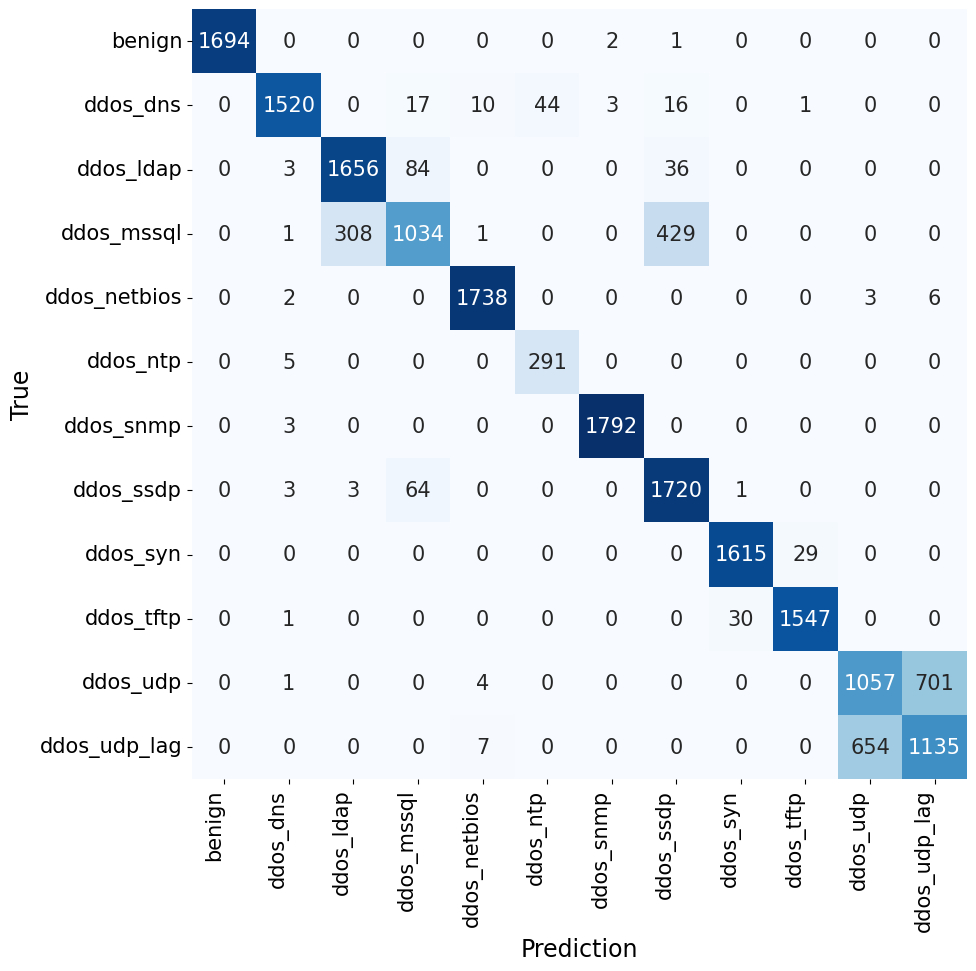
\includegraphics[width=.47\linewidth]{img/heatmap_confusionMatrix.png}} \quad
	\subfloat[][{Most important features for classification.}\label{fig:featureDependency}]
	{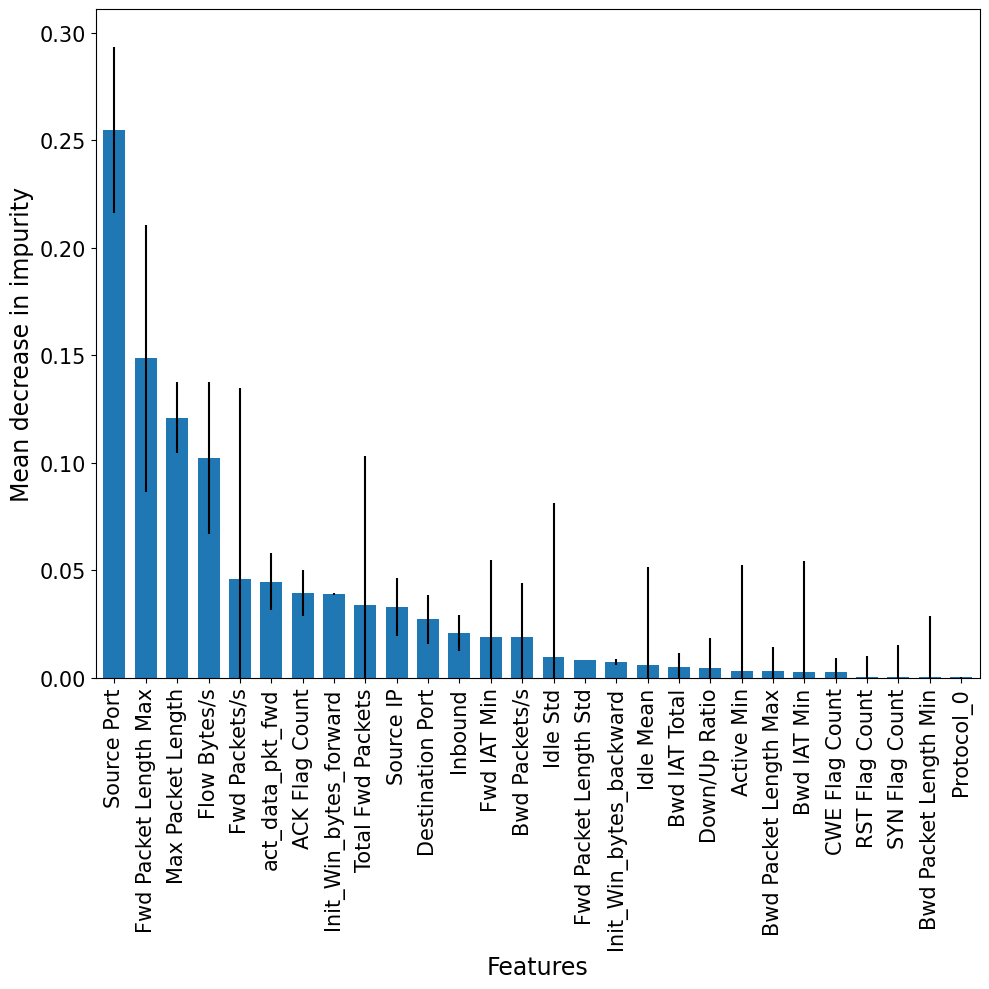
\includegraphics[width=.47\linewidth]{img/barplot_featureDependency.png}} \\
  	\caption{Metrics about the optimized Random Forest.} 
    \Description[Metrics about the optimized Random Forest.]{}
\end{figure}

\section{Unsupervised learning – clustering} \label{sec:unsupervisedLearning}
The goal of this section is to group network flows into clusters that exhibit similar, correlated, or coordinated patterns. A cluster is defined as a group of discrete items that are close to each other. Therefore, the objective of clustering is to identify groups of similar data points that are in some sense homogeneous.
Unlike Section 2, this analysis is performed in an unsupervised manner, independently of the attack labels. In \cref{sec:clusterExplainability}, we will investigate whether distinct `families' or `groups' of attacks naturally emerge based on the features retained in the dataset.
\subsection{Clustering algorithms}
\subsubsection{Algorithms description}
We have decided to perform our analysis using three different algorithms:
\begin{itemize}
    \item k-Means: a hard clustering algorithm, in which each data point is assigned to a single cluster (among the k available clusters). In this algorithm, each cluster is associated with a point (called \emph{mean} or \emph{centroid}).
    \item Gaussian Mixture Model (GMM): a soft clustering algorithm. In this technique, each data is associated with the degree of belonging to each cluster, which can be interpreted as the probability that the i-th data-point belongs to the cluster c. In GMM, each cluster is represented as a random multidimensional Gaussian distribution with its own mean, standard deviation, and covariance. 
    \item DBSCAN: a hard clustering algorithm based on connectivity clustering; data points need to be connected to core points defined as the ones having a minimum number of neighbors.
\end{itemize}

\subsubsection{Performance metrics and indicators}
In order to determine the best algorithm, the best hyper-parameters and the number of clusters, we used several metrics:
\begin{itemize}
    \item Silhouette: measures the consistency within clusters of data, indicating how similar a data point is to its own cluster (cohesion) compared to other clusters (separation). It is defined for each sample by using two values: the mean distance between the sample and all the other points in the cluster, and the mean distance between the samples and all the other points in the next nearest cluster.
    %\[ s = \frac{(b-a)}{max\left(a,b\right)} \]
    \item Rand Index (RI): measures the similarity between two assignments.
    \item Adjusted Rand Index (ARI): corrects the RI ensuring to obtain values close to 0.0 for a random labelling.
\end{itemize}

\begin{figure}
	\centering
    \subfloat[][{Silhouette k-Means.}\label{fig:silKMeans}]
	{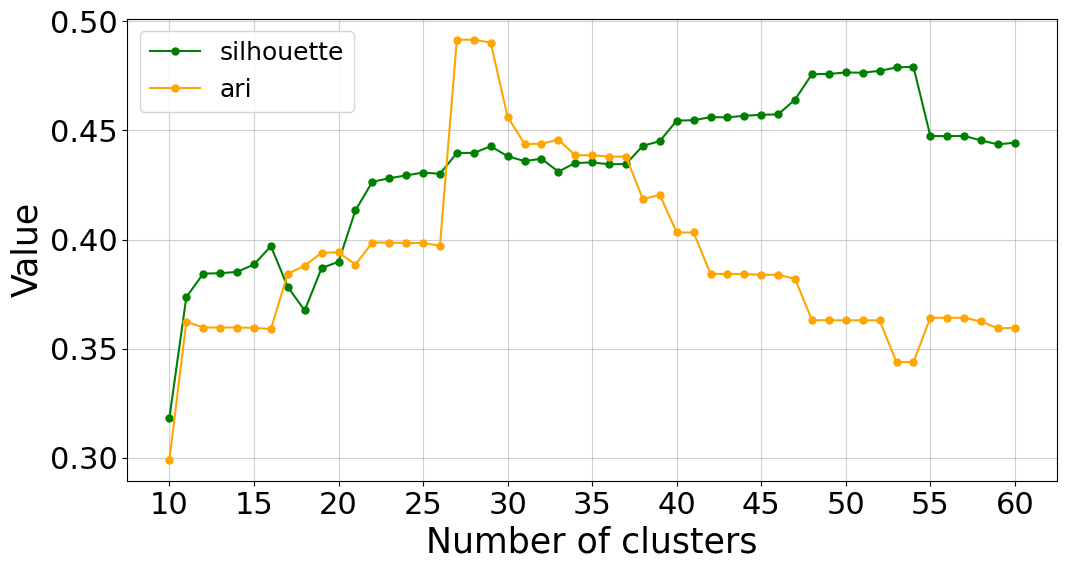
\includegraphics[width=.48\linewidth]{img/scatterplot_kmeansPerfomances.png}} \quad
    \subfloat[][{Silhouette GMM.}\label{fig:silGMM}]
	{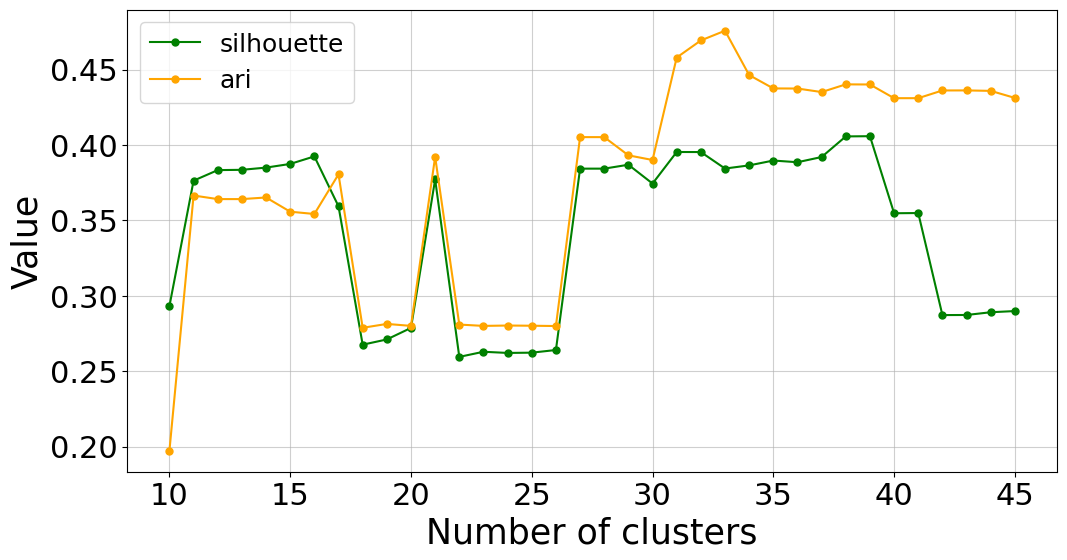
\includegraphics[width=.48\linewidth]{img/scatterplot_gmmPerfomances.png}} \quad   
  	\caption{Hyperparameter tuning k-Means and GMM.} 
    \Description[hyperparameter tuning k-Means and GMM.]{}
    \label{fig:silhouettes}
\end{figure}

\subsection{First algorithm: k-Means}
\subsubsection{Initial parameters and performance}
For the k-Means algorithm, we have only analyzed the \emph{n\_clusters} parameter, which indicates the number of clusters to be created. Regarding the \emph{init} hyper-parameter, we left the default option \verb|k-means++| because it makes centroids to be equally distant from each other, thus leading to better results.
Initially, we set $\emph{n\_clusters}=12$, which is the number of labels.
From this initial analysis, we obtained a silhouette score of 0.38, a RI of 0.81 and an ARI of 0.36, which can be considered as an acceptable starting point: clusters are fairly separated, and they somehow reflect the GT labels. The RI value is not really meaningful, since it can look good simply by random chance. Three of the detected clusters have almost no samples inside, likely representing outliers.
\subsubsection{Hyper-parameter tuning}
Next, we want to see if the previous results can be improved. By varying \emph{n\_clusters}, as shown in \cref{fig:silKMeans}, we observed that the best possible value in terms of the silhouette is 0.48, which can be obtained with $\emph{n\_clusters}=54$. The values for the other metrics are: Clustering Error~$=162121$, RI~$=0.91$ and ARI~$=0.34$. It is evident that the silhouette score notably increased, hence the clusters are now quite separated. On the other hand, increasing the number of clusters does not boost the ARI: in particular, the highest value (0.49) is obtained using 28 clusters, with a silhouette score of 0.44. The clustering error, used only for the k-Means analysis, favors high values of \emph{n\_clusters}: by increasing the number of clusters the average distance from the points to the corresponding cluster means (which defines the clustering error) cannot decrease. Therefore, it is better to focus on the other metrics when evaluating the performance of this algorithm. 

\begin{figure}
	\centering
    \subfloat[][{t-SNE Projection original labels (GT).}\label{fig:tSNEKMeansoriginal}]
	{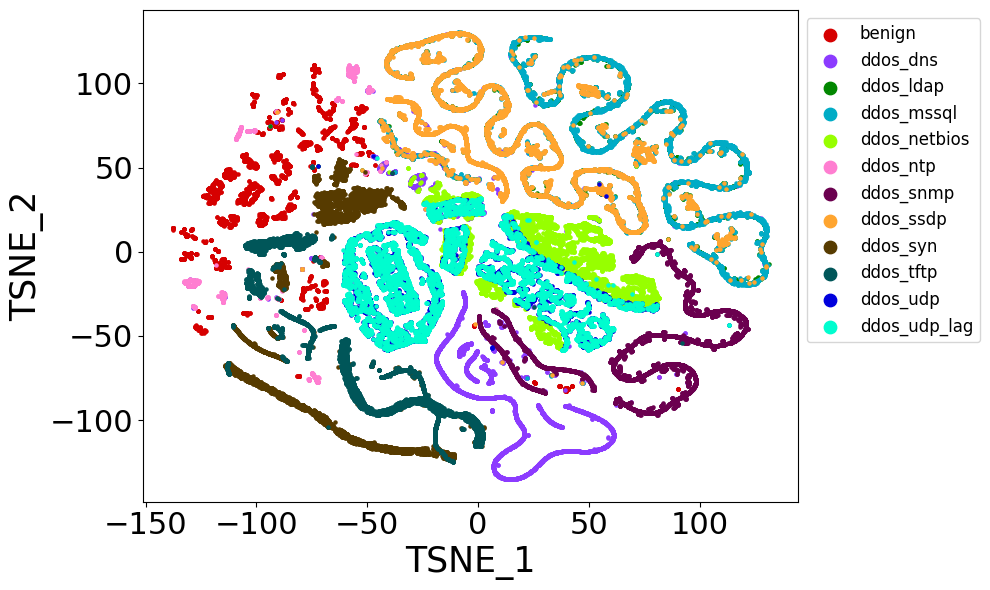
\includegraphics[width=.48\linewidth]{img/tSNE_GT.png}} \quad
    \subfloat[][{t-SNE Projection Plot k-Means 28 clusters.}\label{fig:tSNEKMeansBest}]
	{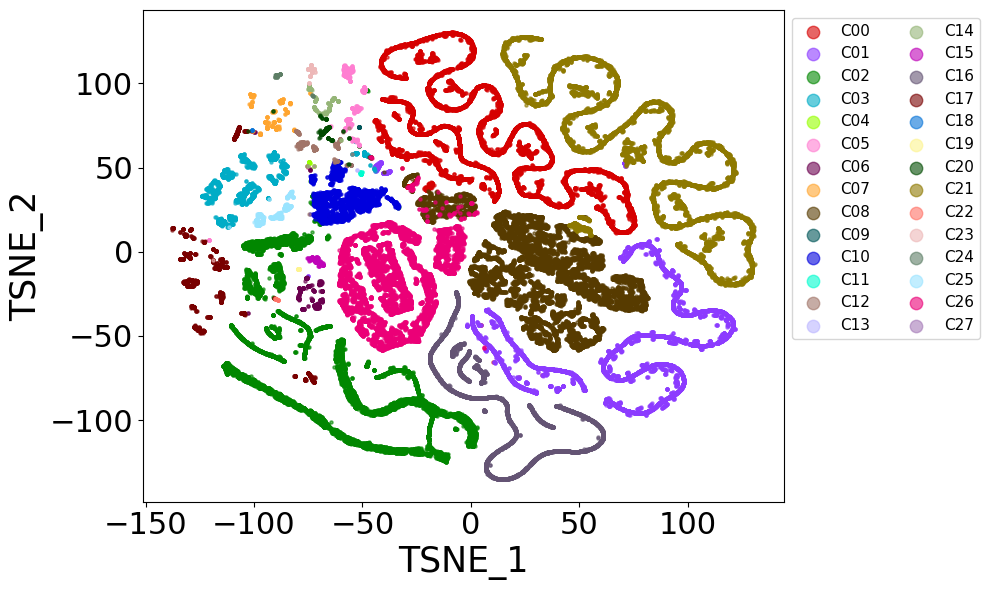
\includegraphics[width=.48\linewidth]{img/tSNE_KMeansBest.png}} \quad
    \subfloat[][{t-SNE Projection Plot GMM 33 clusters.}\label{fig:tSNEGMMbest}]
	{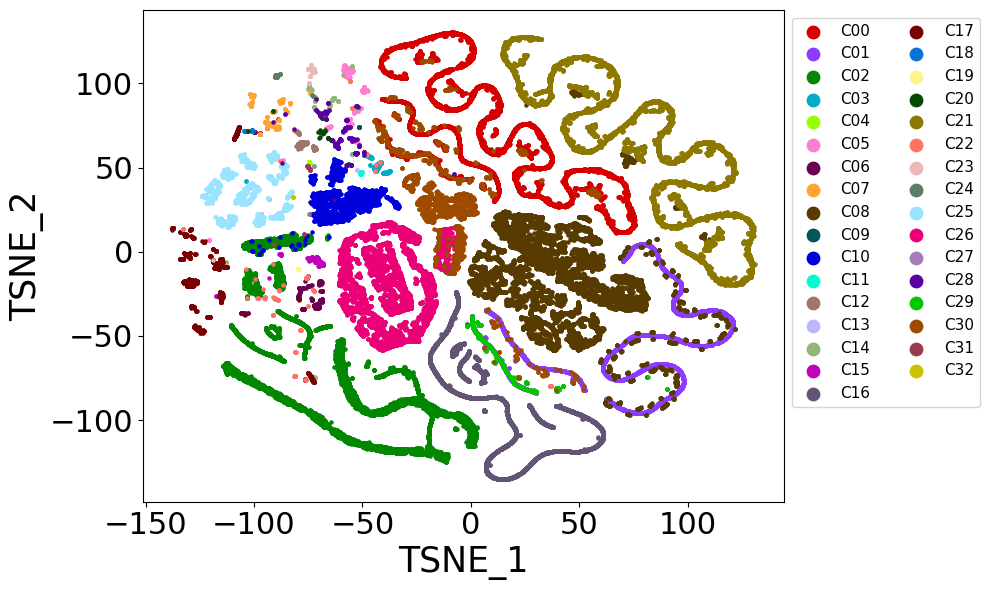
\includegraphics[width=.48\linewidth]{img/tSNE_GMMBest.png}} \quad
    \subfloat[][{t-SNE Projection DBSCAN best parameters.}\label{fig:tSNE_DBSCANbest}]
	{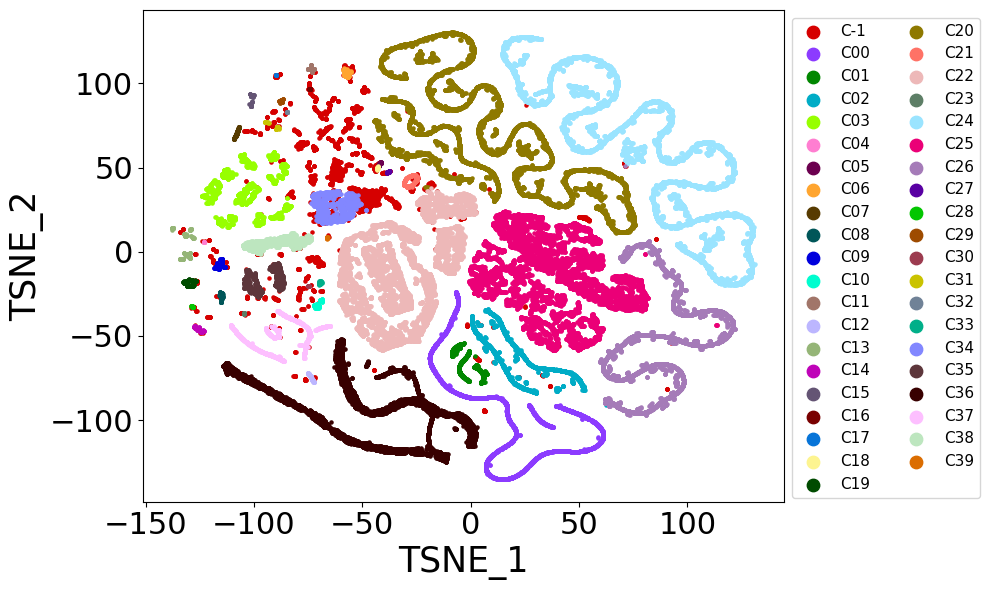
\includegraphics[width=.48\linewidth]{img/tSNE_DbscanBest.png}} \quad
  	\caption{t-SNE Projection Plots.} 
    \Description[t-SNE Projection Plot.]{}
    \label{fig:tSNEProjections}
\end{figure}

\subsubsection{Cluster Visualization and further analysis}
To visualize the obtained clusters we use t-SNE (t-distributed Stochastic Neighbor Embedding), which is a powerful technique for dimensionality reduction and data visualization. 
The \emph{perplexity} hyperparameter is important for the t-SNE algorithm, as it controls the effective number of neighbors that each point considers during the dimensionality reduction process. 
We ran a loop to calculate the Kullback-Leibler (KL) Divergence metric between the high and low-dimensional probability distributions, on various \emph{perplexity} values from 5 to 120 with a 5-point gap, noticing that it becomes quite constant after 100. We also tried to visualize clusters using different \emph{perplexity} values, and we observed that with 50 and 115 the results were pretty similar. We selected a \emph{perplexity} value of 50, as the documentation suggests that typical values are between 5 and 50. At this point, we can visualize the 28 clusters obtained in \cref{fig:tSNEKMeansBest}. This is the clustering that best reflects the labels, leading to the highest ARI. It is evident that the clusters reflect the classes quite well, even though the model groups together \emph{ddos\_netbios} and \emph{ddos\_udp\_lag} samples and it does not discern \emph{ddos\_udp} and \emph{ddos\_udp\_lag}, as well as \emph{ddos\_mssql} and \emph{ddos\_ssdp}. The \emph{benign} traffic is scattered among many different clusters. A more in-depth analysis will be conducted in section \cref{sec:clustersAnalysis}.

\subsection{Second algorithm: Gaussian mixture model (GMM)}
\subsubsection{Initial parameters and performance}
As regards the GMM algorithm, we analyzed the \emph{n\_components} parameter, which indicates the number of clusters to be used.  We set $\emph{n\_components}=12$, which is the number of labels. From this initial analysis, we obtained a silhouette score of 0.38, a RI of 0.81, and an ARI of 0.36. As with k-Means, three clusters are nearly empty, while the first two contain different types of traffic.

\subsubsection{Hyper-parameter tuning}
By varying \emph{n\_components}, as shown in \cref{fig:silGMM}, we observed that the best possible value in terms of silhouette is 0.405, which can be obtained with $\emph{n\_components}=39$. The other metrics are RI $=0.87$ and ARI $=0.44$, that are slightly lower than those obtained with k-Means. The best ARI (0.476) is achieved using 33 clusters, with a silhouette score of 0.38. 
In \cref{fig:tSNEGMMbest} we visualize the clusters obtained with GMM using $\emph{n\_components}=33$: the clustering obtained is quite similar to the one obtained with k-Means, but \emph{ddos\_snmp}, \emph{ddos\_tftp} and \emph{ddos\_ssdp} are divided into more clusters.

\begin{figure}
	\centering
    \subfloat[][{Silhouette DBSCAN.}\label{fig:dbscanSilhouette}]
	{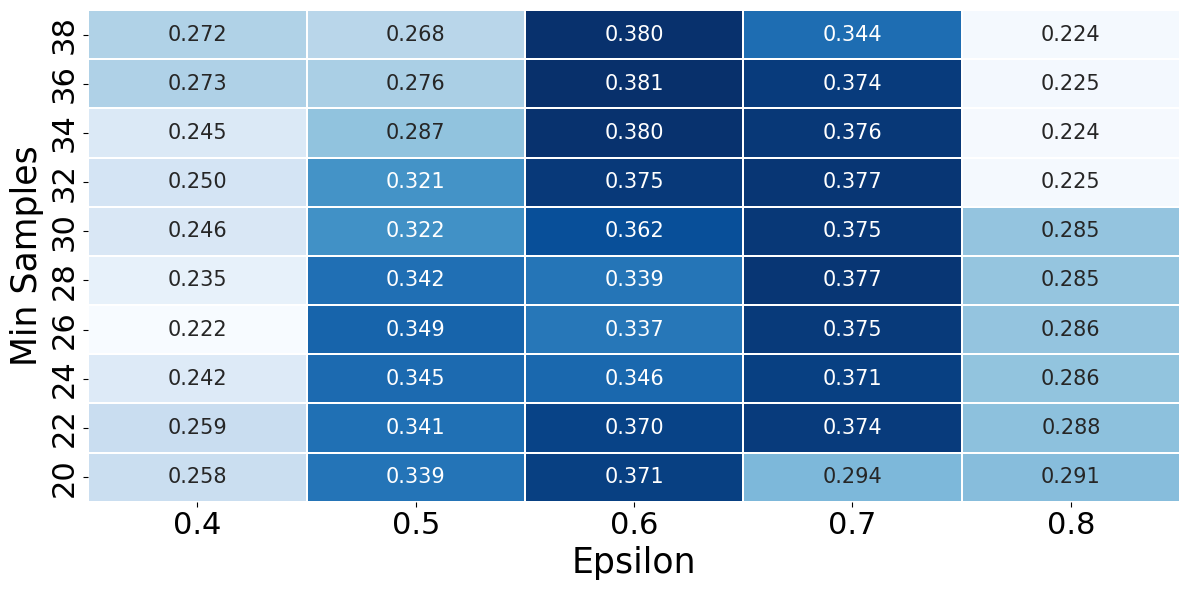
\includegraphics[width=.48\linewidth]{img/dbscanSilhouette.png}} \quad
    \subfloat[][{ARI DBSCAN.}\label{fig:dbscanARI}]
	{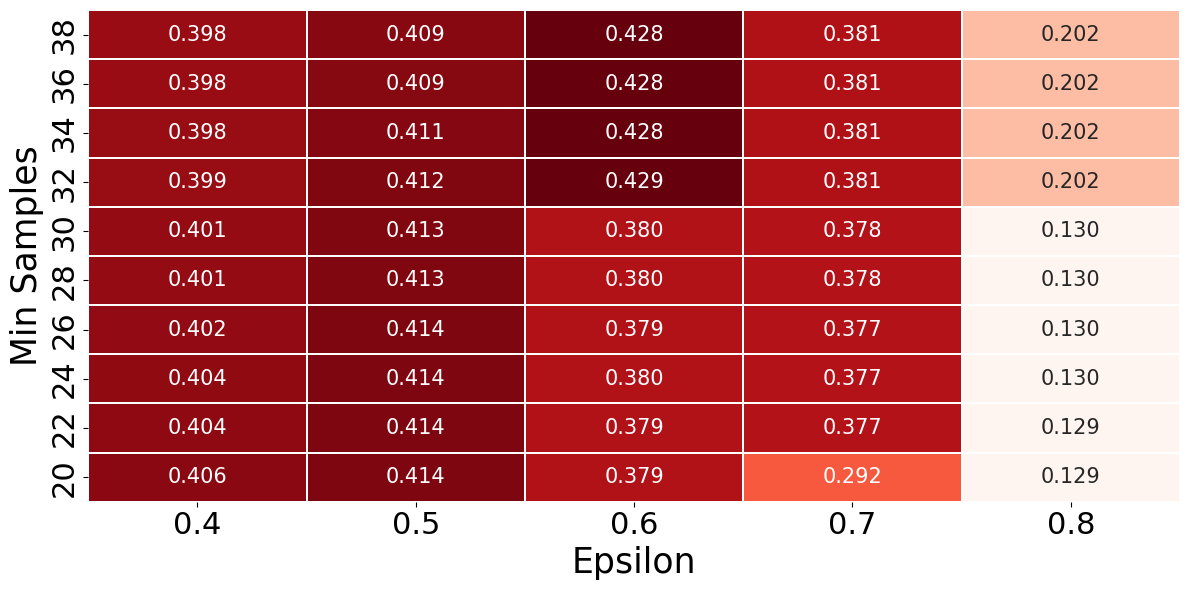
\includegraphics[width=.48\linewidth]{img/dbscanARI.png}} \quad   
  	\caption{Hyperparameter tuning DBSCAN.} 
    \Description[Hyperparameter tuning DBSCAN.]{}
    \label{fig:DBSCAN_scatPlot}
\end{figure}

\subsection{Third algorithm: DBSCAN}
\subsubsection{Initial parameters and performance}
The DBSCAN algorithm autonomously detects the optimal number of clusters, but we need to optimize two parameters by performing a Grid Search: \emph{eps}, which represents the maximum distance within which two points are considered connected, and \emph{min\_samples}, which defines the minimum number of neighbors required for a point to be qualified as a core point. Using default parameters, we obtained a low silhouette score (0.12) and a low ARI (0.26), with 150 clusters and 2144 noise points.

\subsubsection{Hyper-parameter tuning}
Initially, we optimized the silhouette score individually for the two parameters, keeping all other parameters at their default values. We focused on smaller values of \emph{eps}, as larger values significantly slow down the analysis. Subsequently, we conducted a more detailed search around the identified optimal values for \emph{eps} and \emph{min\_samples}. 
The results are presented in \cref{fig:DBSCAN_scatPlot} using two heatmaps that illustrate the variation in silhouette scores and ARI. Overall, the best parameter values we obtained are $\emph{eps}=0.6$ and $\emph{min\_samples}=36$, leading to a silhouette score of $0.38$, ARI $=0.43$, 41 clusters detected, and 4575 noise points. We visualize the resulting clusters in \cref{fig:tSNE_DBSCANbest} using t-SNE: the outcome is similar to those obtained with the other models, but part of \emph{benign} and \emph{ddos\_syn} traffic is classified as noise.

\section{Clusters explainability and analysis} \label{sec:clusterExplainability}
\label{sec:clustersAnalysis}
From the previous section, we can conclude that the k-Means algorithm delivers the best performance. Consequently, we will focus our further analysis on this model, using both 12 and 28 clusters, which correspond to the number of labels and to the option that leads to the best ARI, respectively. In particular, throughout this section we will provide a deeper analysis of the clusters detected, using also the GT labels. Furthermore, we will detect the most important features for our model using permutation importance. Finally, we will identify the sub-attacks and investigate why some attacks are confused by our model. 
\begin{figure}
	\centering
    \subfloat[][{k-Means with 12 clusters.}\label{fig:ECDFclasses_12_clusters}]
	{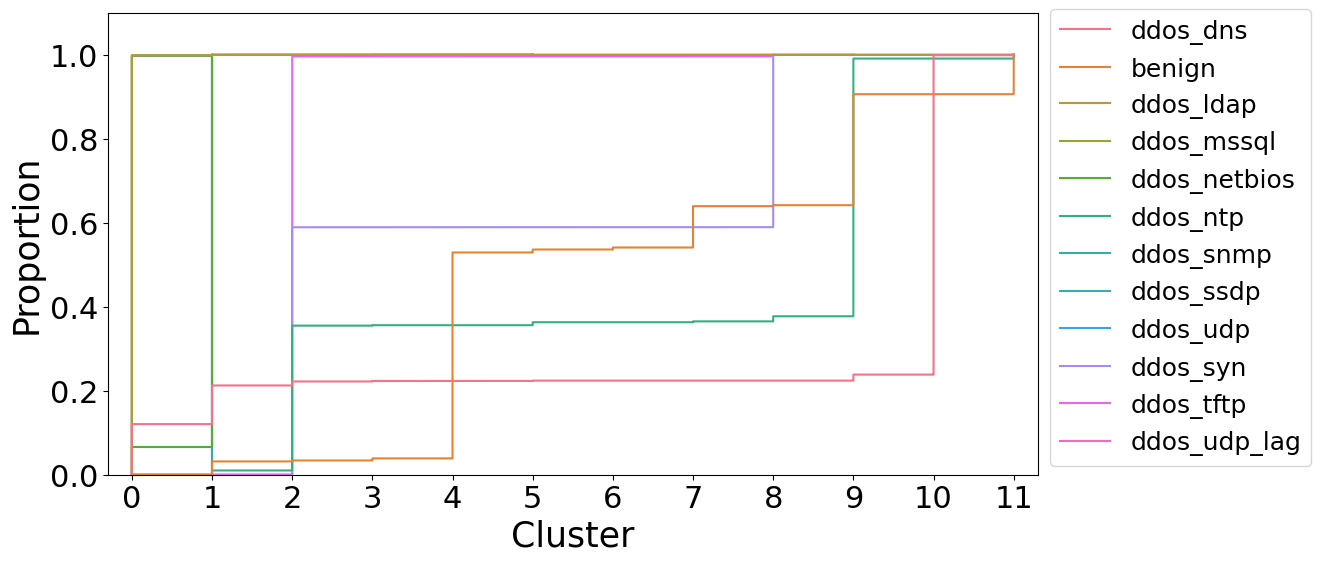
\includegraphics[width=.48\linewidth]{img/ecdf_clusters12.png}} \quad
	\subfloat[][{k-Means with 28 clusters.}\label{fig:ECDFclasses_28_clusters}]
	{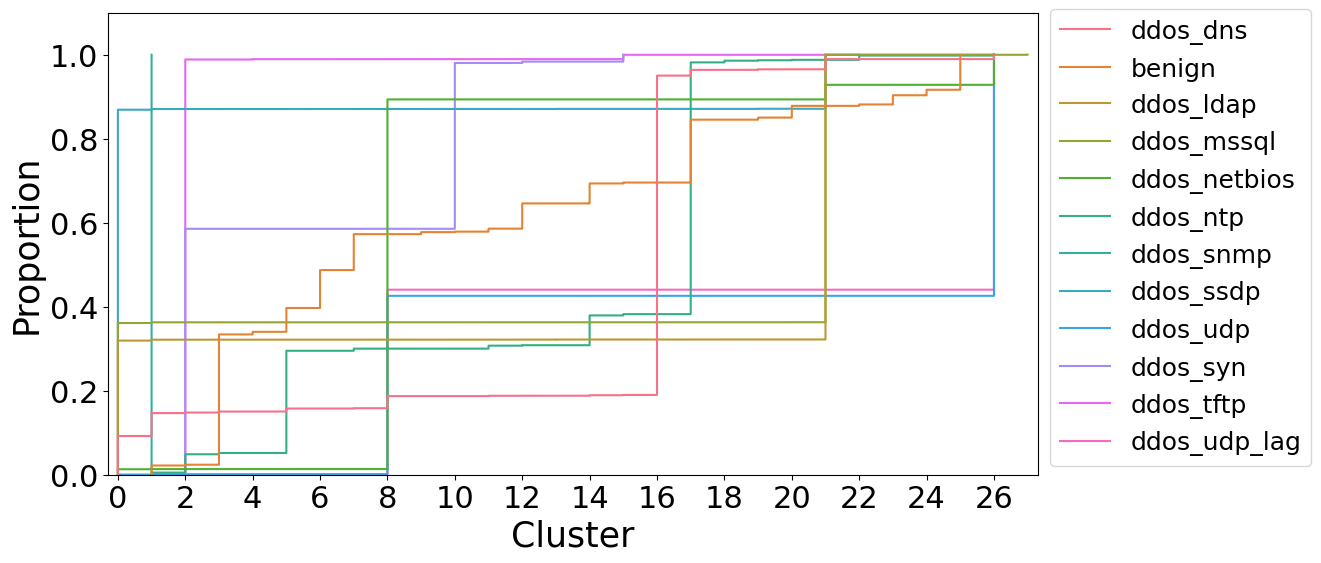
\includegraphics[width=.48\linewidth]{img/ecdf_clusters28.png}} \\
  	\caption{Number of clusters assigned to each class.}  \label{fig:ECDFclasses_clusters}
    \Description[number of clusters assigned to each class.]{}
\end{figure}

\begin{figure}
	\centering
    \subfloat[][{k-Means with 12 clusters.}\label{fig:barplot_classes_12_clusters}]
	{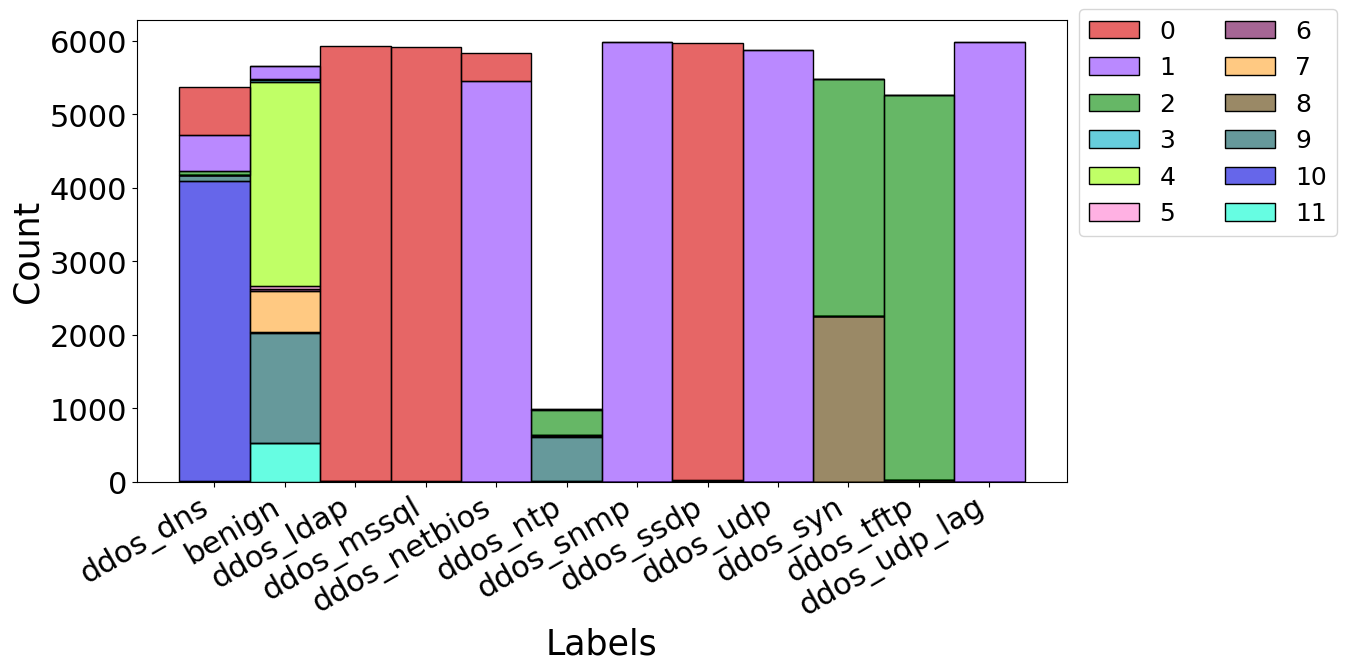
\includegraphics[width=.48\linewidth]{img/barplot_clusters12.png}} \quad
	\subfloat[][{k-Means with 28 clusters.}\label{fig:barplot_classes_28_clusters}]
	{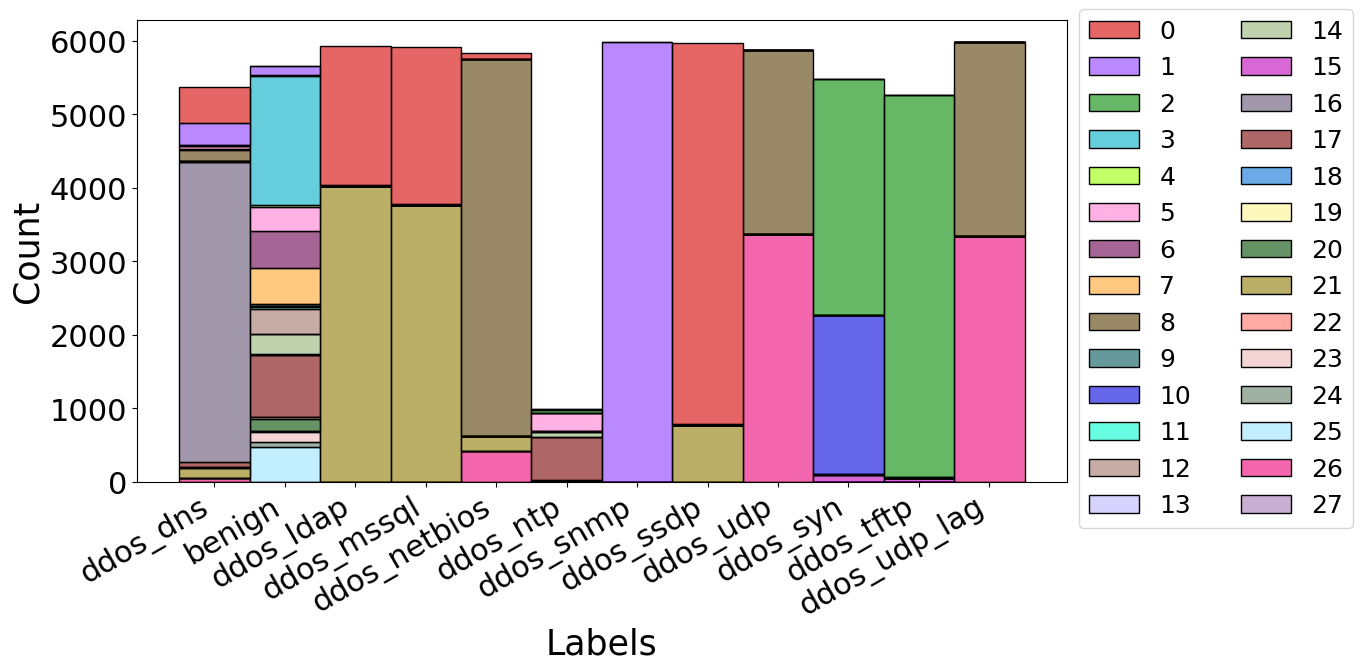
\includegraphics[width=.48\linewidth]{img/barplot_clusters28.png}} \\
  	\caption{Attacks distribution between clusters.} 
    \label{fig:barplot_classes_clusters}
    \Description[Attacks distribution between clusters.]{}
\end{figure}
\subsection{Cluster distribution of traffic types}
We may think that the detected clusters reflect more or less the labels of our samples. However, real traffic is more complex and, as already seen in \cref{sec:supervisedLearning}, models struggle to classify certain types of attacks. \Cref{fig:ECDFclasses_clusters} represents the ECDF of number of clusters assigned to each class, while \cref{fig:barplot_classes_clusters} visualizes how samples of each attack are distributed among clusters. In particular, from \cref{fig:ECDFclasses_12_clusters} and \cref{fig:barplot_classes_12_clusters}, it is evident that approximately all samples of some attacks are assigned to the same cluster: \emph{ddos\_netbios}, \emph{ddos\_snmp}, \emph{ddos\_udp}, and \emph{ddos\_udp\_lag} flows are all included in cluster 1, while those of \emph{ddos\_ldap}, \emph{ddos\_mssql} and \emph{ddos\_ssdp} belong to cluster 0. All \emph{ddos\_tftp} samples and half of the \emph{ddos\_syn} ones are in cluster 2. On the other hand, \emph{benign} traffic is scattered among different clusters, meaning that it presents many different patterns: clusters 4, 7 and 11 are characteristic of harmless flows, while more than a thousand samples are assigned to cluster 9, which also contains \emph{ddos\_ntp} traffic. Hence, they may have some common elements, since also the SVM model tends to confuse them (\cref{sec:svm}). \emph{ddos\_dns} is probably quite different from the others attacks, since the majority of its samples are assigned to cluster 1, that contains only this type of traffic. Looking at \cref{fig:ECDFclasses_28_clusters} and \cref{fig:barplot_classes_28_clusters}, we can notice that the model still confuses the same classes of before, but the samples of many attacks are now divided into two or more clusters, suggesting the presence of sub-attacks. For instance, \emph{ddos\_ldap}, \emph{ddos\_mssql} and \emph{ddos\_ssdp} are split into a couple of clusters and the first two also in the same proportion. Same thing for \emph{ddos\_udp}, \emph{ddos\_udp\_lag} and \emph{ddos\_netbios}. On the other hand, \emph{ddos\_snmp} flows now belong to a completely different cluster. The \emph{benign} class is still scattered among different clusters, but mantains cluster 17 in common with \emph{ddos\_ntp}. Moreover, \emph{ddos\_syn} flows are still split into two clusters, so it has two main sub-attacks. Finally, \emph{ddos\_tftp} traffic is still clustered together: its traffic is very homogeneous.

\begin{figure}
	\centering
    \subfloat[][{Permutation feature importance.}\label{fig:featureImportance28cluster}]
	{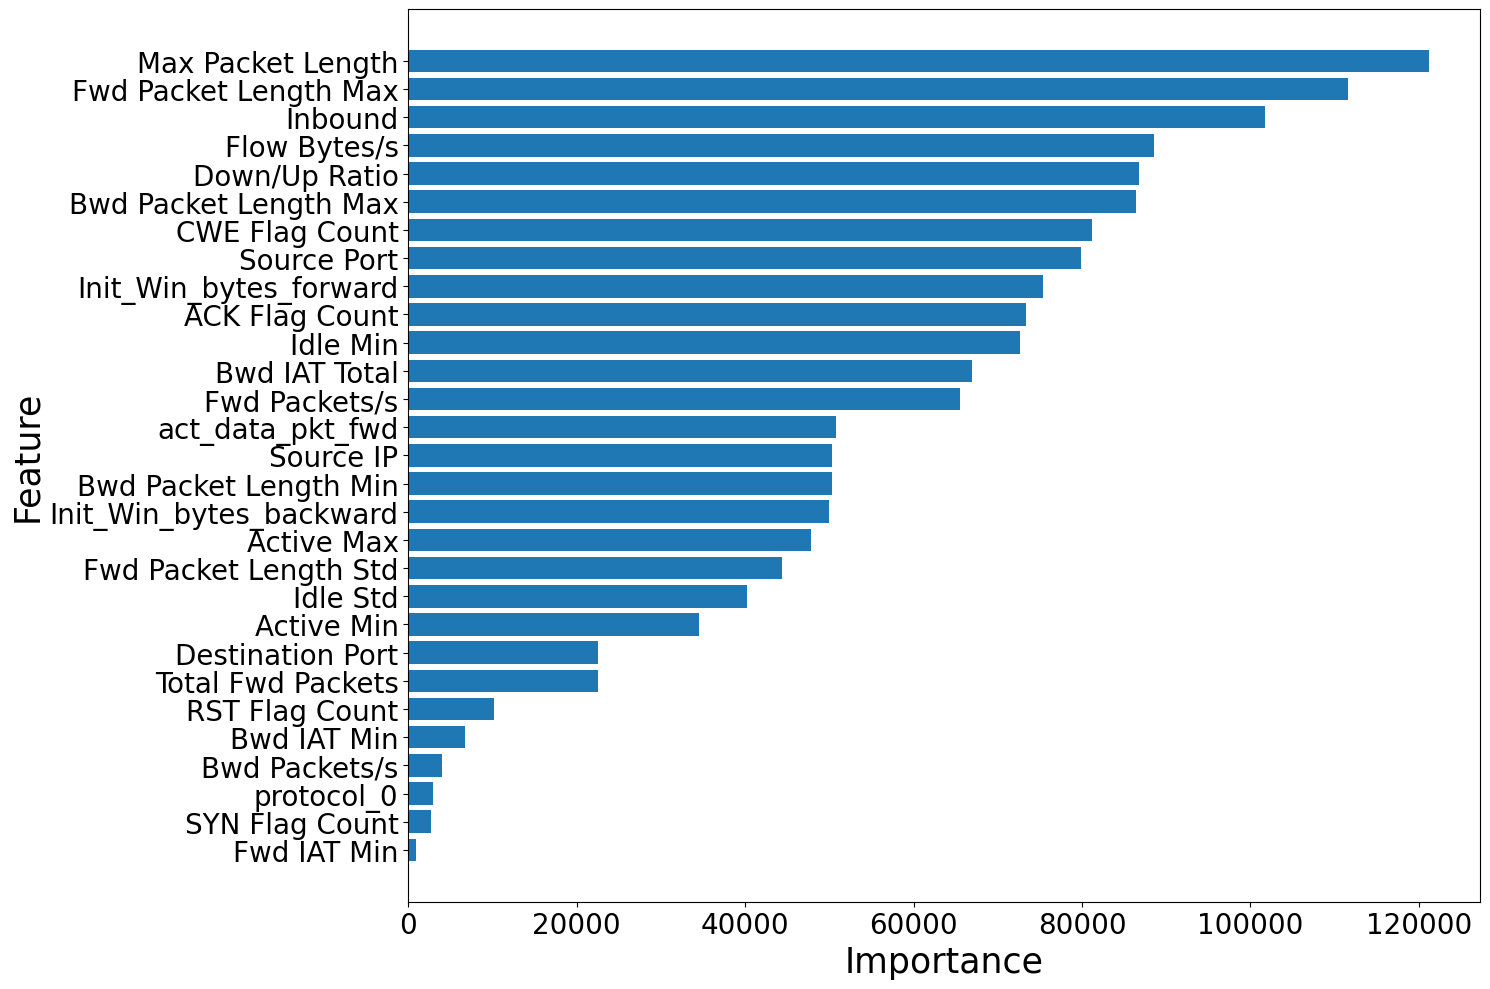
\includegraphics[width=.48\linewidth]{img/featureImportance28cluster.png}} \quad
	\subfloat[][{Permutation feature importance correlated features.}\label{fig:featureImportance28clusterMinimal}]
	{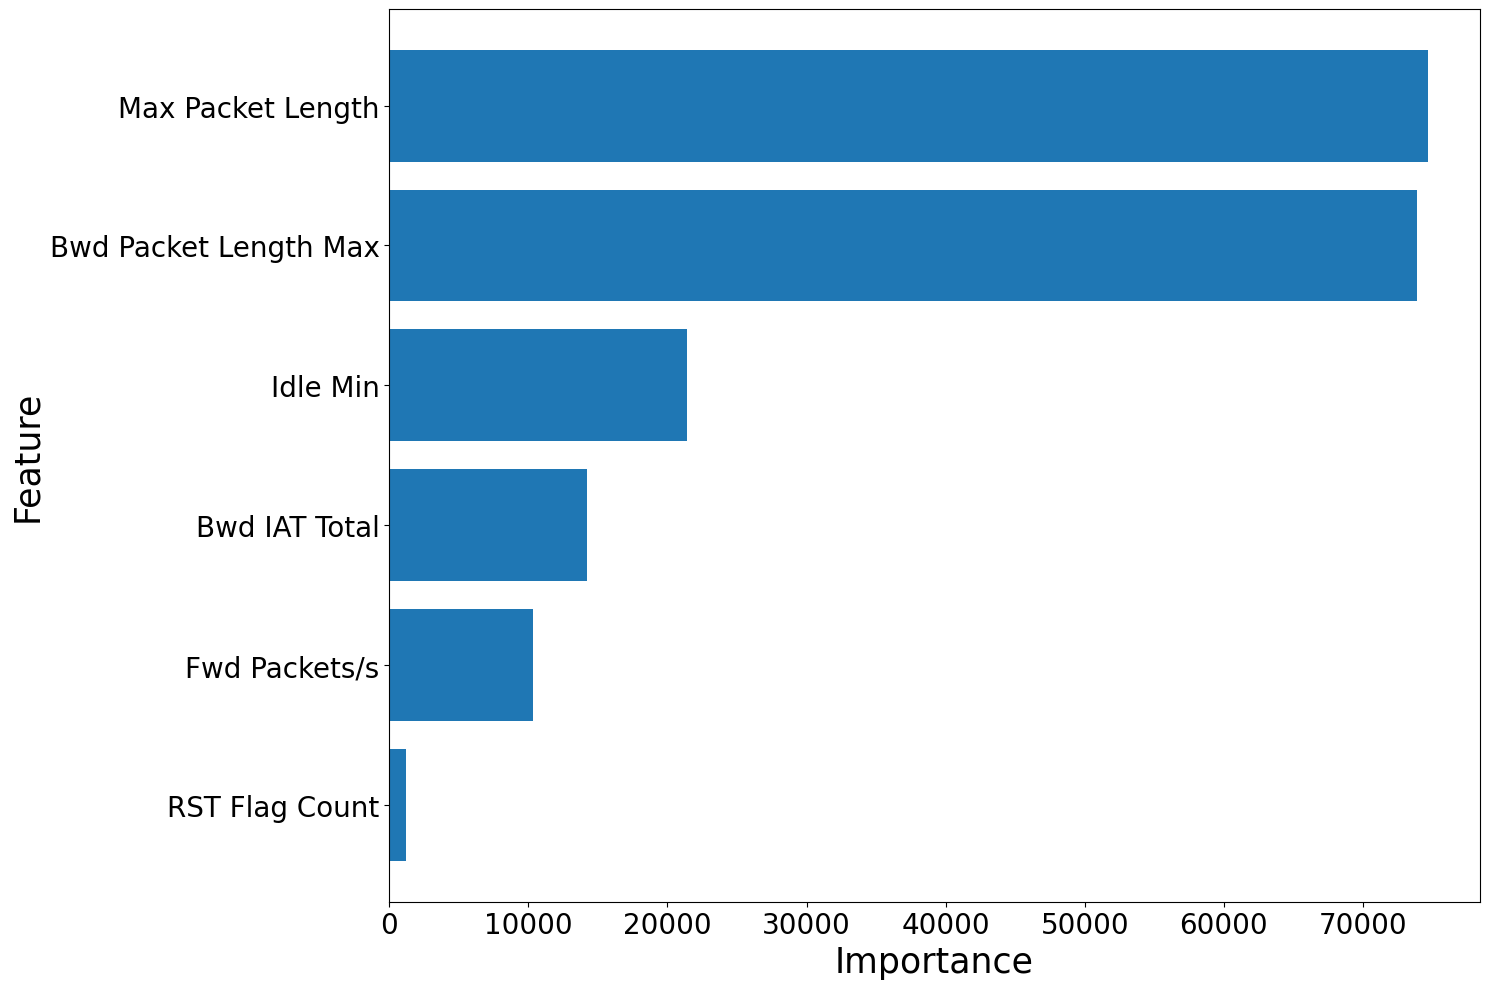
\includegraphics[width=.48\linewidth]{img/featureImportance28clusterMinimal.png}} \\
  	\caption{Feature importance on k-Means with 28 clusters.} 
    \Description[Feature importance on k-Means with 28 clusters.]{}
\end{figure}

\subsection{Feature importance analysis}\label{sec:featureImportanceUL}
In this section, we attempt to detect the most important features in the trained model. For this purpose, we used the permutation feature importance: this technique consists in taking a feature and randomly shuffling its values, breaking any kind of relationship between that feature and the result. Then, it applies the already trained model to the dataset with these shuffled features: if performance decreases significantly compared to the one with the original dataset, it means that that feature is really important to our model. \Cref{fig:featureImportance28cluster} shows the outcome of this technique applied to the k-Means model with 28 clusters. The most important features are \emph{Max Packet Length} and \emph{Fwd Packet Length Max}, while the least ones are \emph{protocol\_0} and \emph{Fwd IAT Min}. \emph{Source IP}, \emph{Source Port} and \emph{Destination Port} are not really important to our model, meaning that it may be able to generalize other data. We also applied this technique to the k-Means model with 12 clusters, obtaining similar results. The \emph{Max Packet Length} was already an important feature for the Random Forest model, as analyzed in \cref{sec:resultInvestigation}.

Even though we already performed dimensionality reduction during the preprocessing phase, there are still quite high-correlated features. When features are collinear or highly correlated, permuting one feature has little effect on the models' performance because it can get the same information from a correlated feature. One way to address this is by performing hierarchical clustering on the Spearman rank-order correlations, picking a threshold, and keeping a single feature from each cluster. Finally, we performed the permutation feature importance using the dataset containing only the selected features. The result is shown in  \cref{fig:featureImportance28clusterMinimal} and it almost reflects the one obtained before.

\subsection{Attack pattern investigation}
In the previous paragraphs, an in-depth analysis has been performed to explain how some attacks might contain sub-attack patterns, as \emph{ddos\_syn}. We can hypothesize that the most important features identified in \cref{sec:featureImportanceUL} are those that make two samples being clustered together or not. Hence, to complete our analysis, we wrote a custom function to detect the most diverse features among two given clusters containing the same label, with the aim of understanding which features contribute to uniquely identifying some particular attack patterns. For instance, we discovered that the most discriminative features for \emph{ddos\_syn} between cluster 2 and cluster 10 are \emph{Destination Port}, \emph{Fwd Packets/s}, and \emph{Flow Bytes/s}. By applying the same function to other clusters and classes, we noticed that in most cases these three features are the most discriminative, along with \emph{Total Fwd Packets}, \emph{Bwd IAT Total} and \emph{Active Max}. This means that the different sub-attacks have different values for those features, so they are classified into different clusters. 

On the other hand, the attacks clustered together have similar values for those features. Therefore, we tried to find the most diverse features between two classes in the same cluster, in order to better understand why flows belonging to different classes are grouped together. In general, results show that even the most different features have quite similar values among the confused classes, meaning that the model struggles to discern them. \emph{Fwd Packets/s}, \emph{Flow Bytes/s}, \emph{Fwd Packet Length Max}, \emph{Source Port}, and \emph{Destination Port} are the most distinctive features, but still too similar.

In conclusion, we analyze similarities between attacks from the perspective of their definition or attack methodology. The \emph{ddos\_ssdp}, \emph{ddos\_ldap} and \emph{ddos\_mssql} attacks are amplification and reflection based: the attacker sends a small command to the accomplices resulting in a large amount of traffic being sent to their victim. Hence, he needs fewer accomplices to overwhelm the victim. Both \emph{ddos\_udp} and \emph{ddos\_udp\_lag} attacks are UDP-based and their goal is to cause a performance degrade. In particular, in UDP flood attack this is achieved by sending numerous UDP packets to random ports at a very high rate, while UDP-LAG attack is mostly used in online gaming where the attacks want to slow down or interrupt the movement of other players to outmaneuver them. Finally, both \emph{ddos\_syn} and \emph{ddos\_tftp} attacks are performed over TCP (\cref{fig:heatmapProtocol}) and aim to consume resources on the victim server.

\section{Conclusions}
In conclusion, supervised and unsupervised ML models allow us to automate the detection and analysis of flows generated during DDoS attacks. In particular, they are able to distinguish benign from malicious traffic, as well as identify the class of attack. However, they are not able to perfectly discern all of them, since some exhibit similar patterns. Using supervised learning techniques, we can predict the correct label with high precision on unseen data. This means that the trained model could be used to classify traffic from future attacks in the same context. On the other hand, unsupervised learning models allow us to group the traffic into different categories that somehow reflect the original labels, although we identified some confused classes and sub-attacks. Therefore, these results can be used to develop effective defenses against DDoS attacks, as well as to study their characteristics and patterns more in depth.

\clearpage
\nocite{*}
\bibliographystyle{unsrt}
\bibliography{bibliography}

\clearpage
\appendix
\section{Correlation matrix using the Pearson correlation coefficient} \label{app:correlationMatrix}
\vfill
{\centering 
    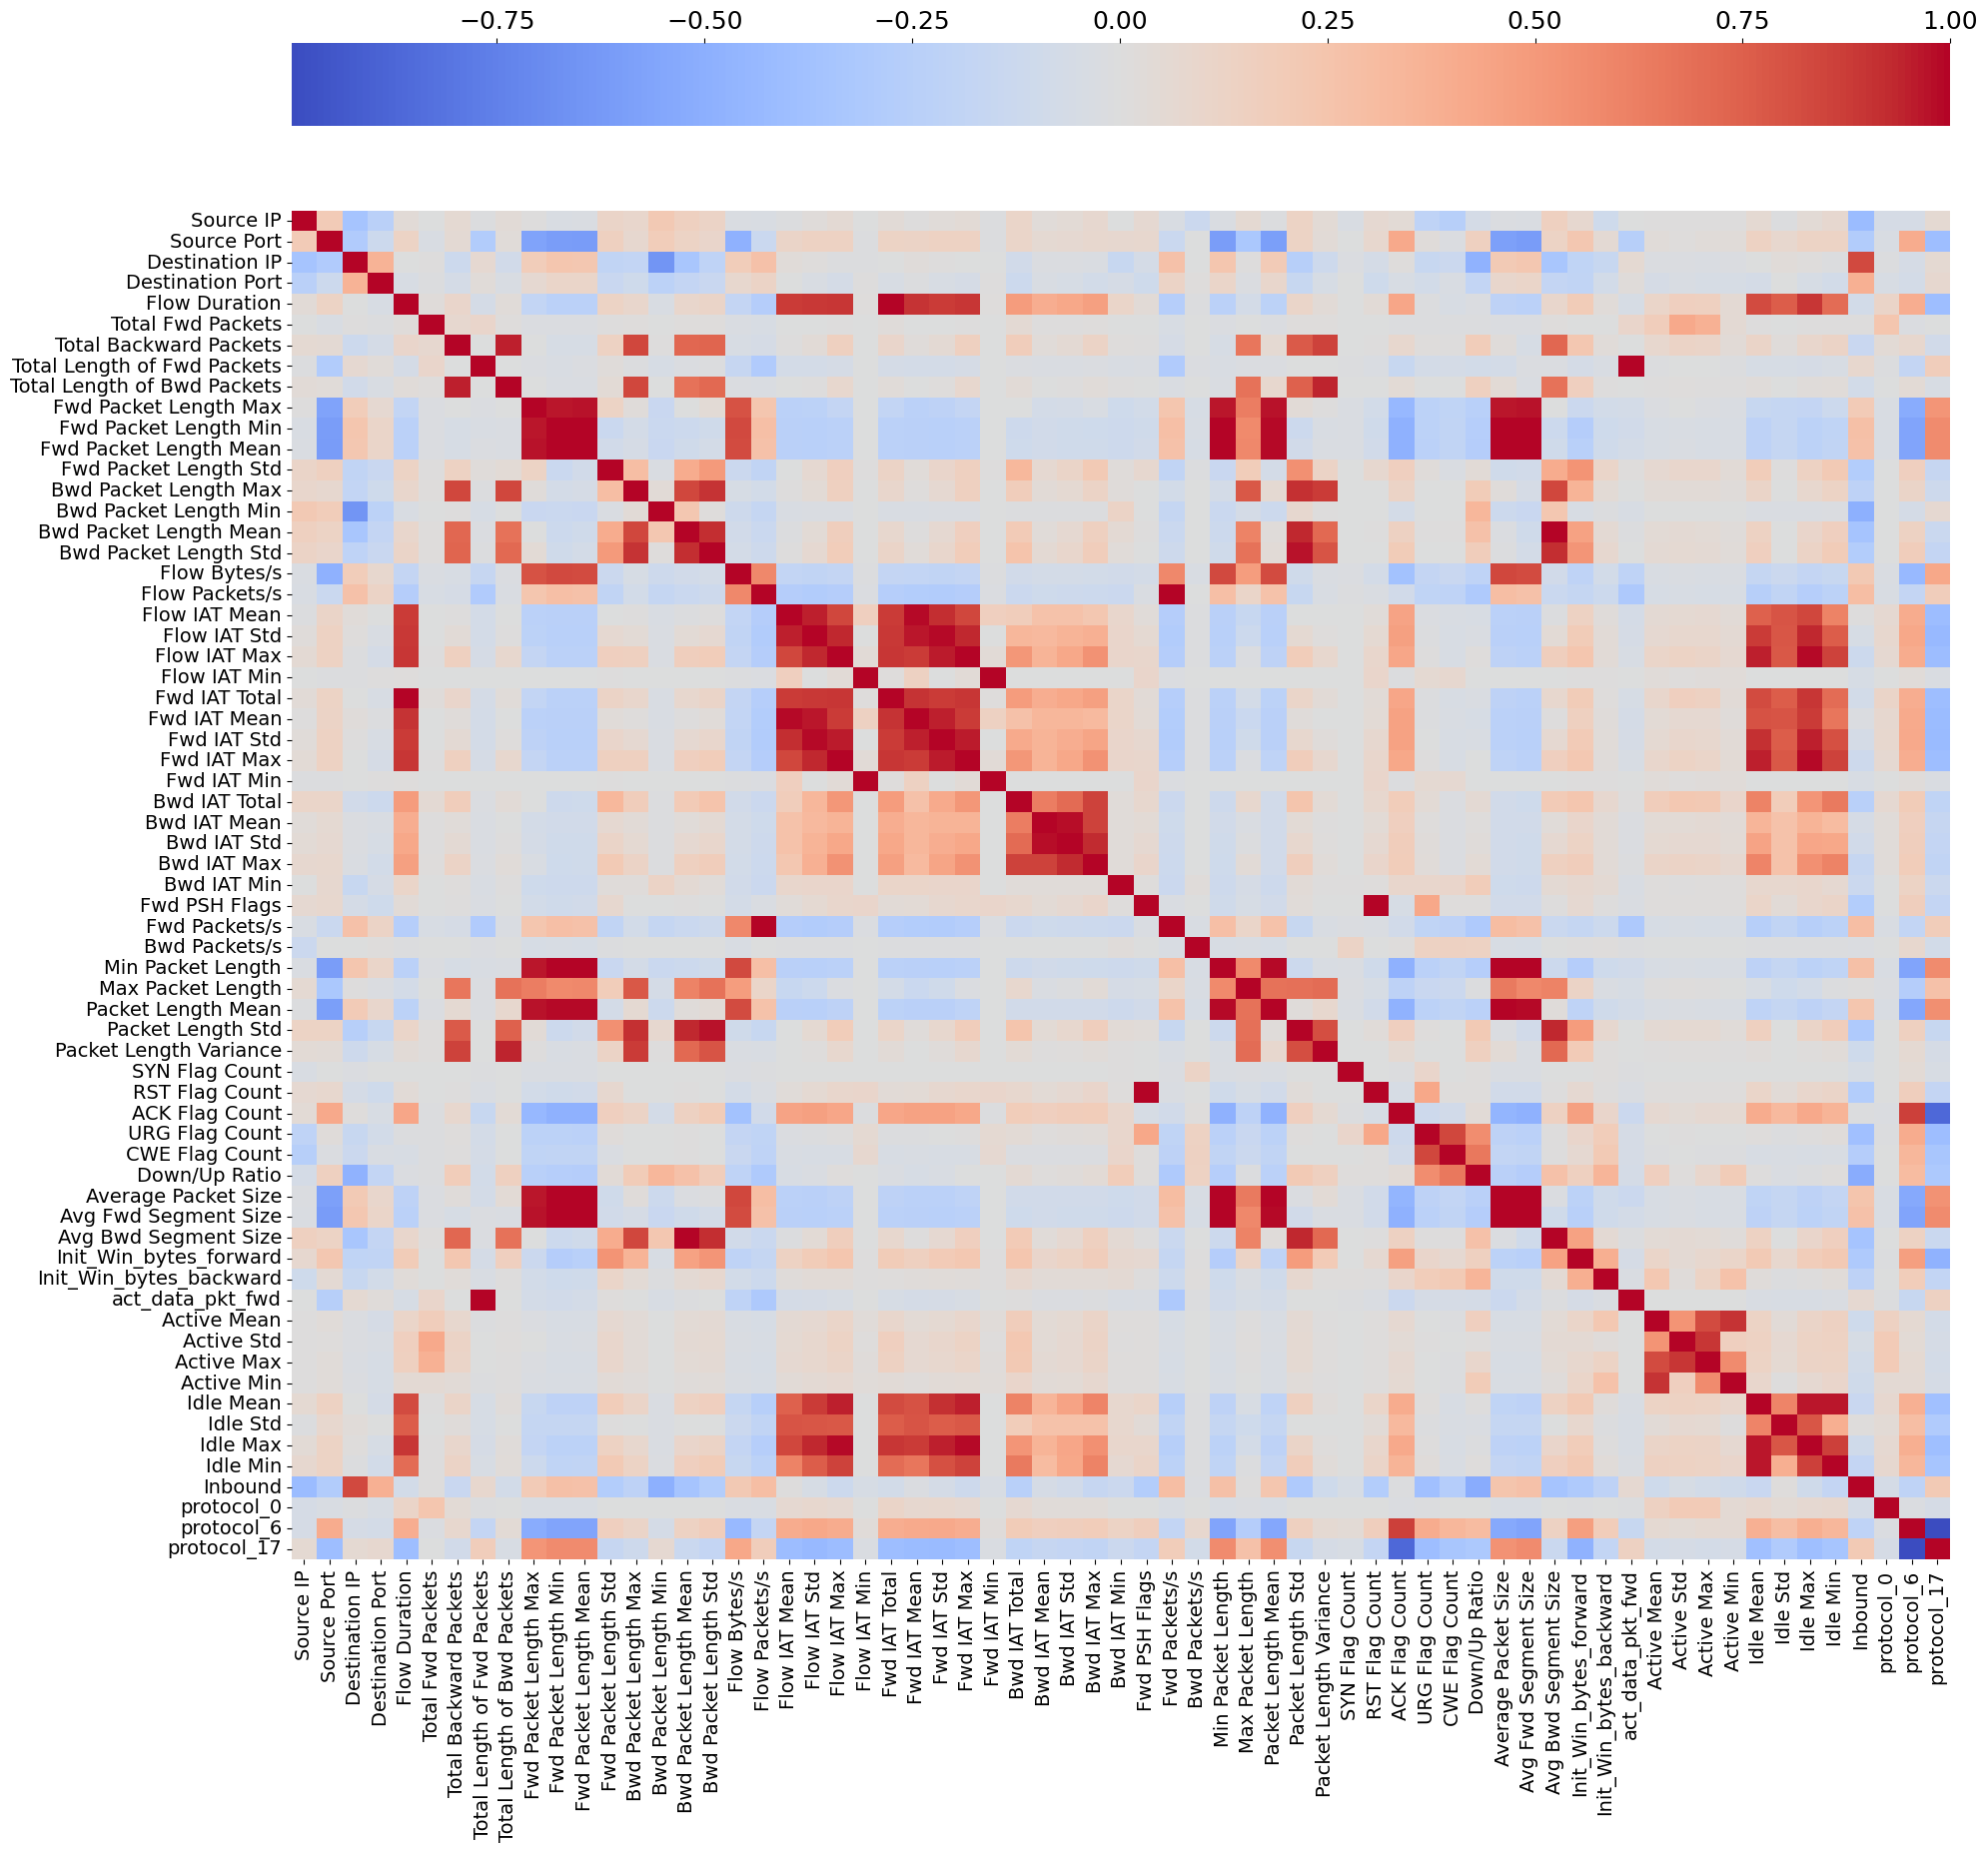
\includegraphics[width=1\linewidth]{img/heatmap_correlationMatrix.png}
}
\vfill

\clearpage
\section{Other supervised learning ML models} \label{app:otherModels}
The objective of this section is to investigate the two techniques of supervised learning that we decided not to talk about in \cref{sec:supervisedLearning}.

\subsection{Naive Bayes Classifier}
Naive Bayes Classifier (Gaussian NB) is a probabilistic model based on Bayes’ theorem, assuming that the features follow a Gaussian (normal) distribution.

\subsubsection{Default model performance evaluation} 
As Logistic Regression, the Naive Bayes Classifier works in the space of linear maps. This probabilistic classifier assumes that the features follow a Gaussian distribution, supposing them to be independent from each other: its goal is to estimate the mean and standard deviation of these distributions. However, the features in our dataset are not completely independent and do not follow a perfect Gaussian distribution; moreover, the model is sensitive to noise and outliers. 

The model exhibits an accuracy of \SI{56}{\percent} in both the training and test sets, suggesting underfitting. We will address this issue during the hyperparameter tuning phase. Additionally, metrics such as precision, recall, and F1-score are quite poor in some classes. In particular, they are zero on both the training and test set for the \emph{ddos\_udp} class, while \emph{ddos\_udp\_lag} has low precision by high recall, since many samples tend to be recognized as this attack by the model (a large amount of false positives impacts precision but not recall). Furthermore, the model struggles to correctly classify \emph{ddos\_ldap}, \emph{ddos\_mssql}, and \emph{ddos\_tftp} samples.

\subsubsection{Hyperparameter tuning and results} 
In the Naive Bayes Classifier we tried to optimize the \emph{var\_smoothing} parameter, which indicates the largest variance of all features that are added to variances for calculation stability. Using $\emph{var\_smoothing}=\num{e-1}$ we obtained an accuracy of \SI{65}{\percent} in both the training and the validation set: after performing the hyperparameter tuning, the class \emph{ddos\_udp} still has zero precision, recall, and F1-scores, while the performances on some other classes, such as \emph{ddos\_mssql} and \emph{ddos\_tftp}, improved. This is the model in which the accuracy improved the most after hyperparameter tuning.

Although the performances of this model are not excellent, it has multiple pros. The main one is its efficiency: both the fit phase took only \SI{0.01}{\second}, while the predict \SI{0.05}{\second}.

\subsection{Support Vector Machines}\label{sec:svm}
Support Vector Machines (SVM) refer to a class of powerful algorithms that find the optimal hyperplane to separate data points of different classes. SVM is particularly effective in high-dimensional spaces and when there is a clear margin of separation between classes. The choice of kernel (e.g., linear, polynomial, or RBF) plays a crucial role in its performance, allowing it to handle both linear and non-linear classification tasks. However, the C-Support Vector Classification algorithm provided in the \verb|sklearn.svm| library does not seem to be the best choice for our dataset, since the fit time scales at least quadratically with the number of samples and may be impractical beyond tens of thousands of samples. Indeed, for large datasets it is suggested to use \verb|LinearSVC|.

\subsubsection{Default model performance evaluation} \hspace{0pt}
In linear SVC, multiclass support is handled according to a one-vs-the-rest scheme. It tries to find a linear hyperplane that separates the data. Using the default parameters, it has an accuracy of \SI{70}{\percent} in both the training and the test sets, suggesting underfitting. In addition to the misclassifications already described in \cref{sec:preliminaryRemarks}, it performs very poorly in the \emph{ddos\_mssql} class, since it often predicts its samples as belonging to \emph{ddos\_ldap}. It also assigns to \emph{ddos\_netbios} class \emph{ddos\_udp} and \emph{ddos\_udp\_lag}. Moreover, it tends to assign malicious traffic (\emph{ddos\_ntp}) to the \emph{benign} class.

\subsubsection{Hyperparameter tuning} 
We tried to optimize:
\begin{enumerate}
    \item \emph{tol}: the tolerance for the stopping criteria.
    \item \emph{C}: a regularization parameter; it is inversely proportional to the size of the margin. By using a smaller value and obtaining a larger margin, the classifier becomes more flexible and allows more classification mistakes. A high value may lead to overfitting.
\end{enumerate}

\subsubsection{Results}
The combination of hyperparameters that leads to the highest accuracy in the validation set (\SI{70}{\percent}) is: $\emph{C}=100$ and $\emph{tol}=\num{e-5}$. The model performance did not improve much after the hyperparameter tuning phase, which means that it is probably not very suitable for classifying our dataset. However, we can highlight that it tends less to classify the \emph{ddos\_ntp} flows as \emph{benign}.

This model has the highest cost among the analyzed models: in particular, the fit phase takes \SI{393.81}{\second} for Linear SVC.

\end{document}

